\documentclass{article}
\usepackage{geometry}
\geometry{a4paper, margin=1in}
\usepackage{amsmath}
\usepackage{graphicx}
\usepackage{longtable}
\usepackage{booktabs}
\usepackage{array}
\usepackage{hyperref}
\usepackage{xcolor}
\usepackage{listings}
\extrafloats{100}

\definecolor{codebackground}{RGB}{247,248,250}
\definecolor{codekeyword}{RGB}{0,76,153}
\definecolor{codecomment}{RGB}{76,120,76}
\definecolor{codestring}{RGB}{163,21,21}
\lstdefinestyle{tracepv}{
    backgroundcolor=\color{codebackground},
    basicstyle=\ttfamily\footnotesize,
    keywordstyle=\color{codekeyword}\bfseries,
    commentstyle=\color{codecomment}\itshape,
    stringstyle=\color{codestring},
    numbers=left,
    numberstyle=\tiny\color{gray},
    stepnumber=1,
    numbersep=8pt,
    frame=single,
    rulecolor=\color{gray!45},
    breaklines=true,
    breakatwhitespace=false,
    showstringspaces=false,
    tabsize=4,
    columns=fullflexible,
    keepspaces=true,
    captionpos=b,
    aboveskip=0.8em,
    belowskip=0.8em
}
\lstset{style=tracepv}

\title{TRACE-PV Workflow}
\date{}
\author{}

\begin{document}
\maketitle

\section*{Workflow Sequence Diagram}
The sequence diagram depicts the workflow of the TRACE-PV simulation process. It begins with the user providing inputs through the GUI, which are collected, validated, and transferred as simulation inputs for model building and mission profile construction. The multi-physics stressor simulator then runs the simulation, generating stressors that are passed as the inputs for the reliability assessment to evaluate component lifetime and calculate the LCOE. Decision logic determines whether any component has reached its end of life (EOL); if so, the system reports the EOL, lifetime, LCOE, and historical stressors of the component, whereas if no component has failed, the simulation continues until the termination criteria are satisfied. Finally, the GUI displays the results and status to the user, completing the simulation sequence.

\begin{figure}[h]
    \centering
    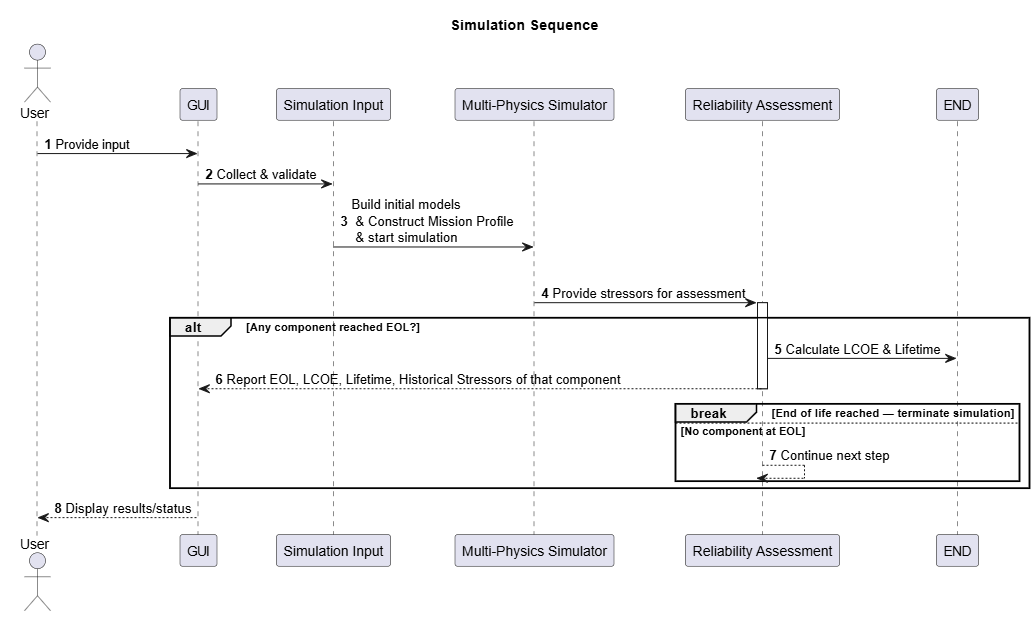
\includegraphics[width=\textwidth]{figure1.png}
    \caption{Workflow Sequence Diagram}
\end{figure}

\section{Simulator Inputs}
The graphics user interface is used to take the required mission profiles, model configurations and necessary information for the reliability assessment for the PV inverter.

\begin{figure}[h]
    \centering
    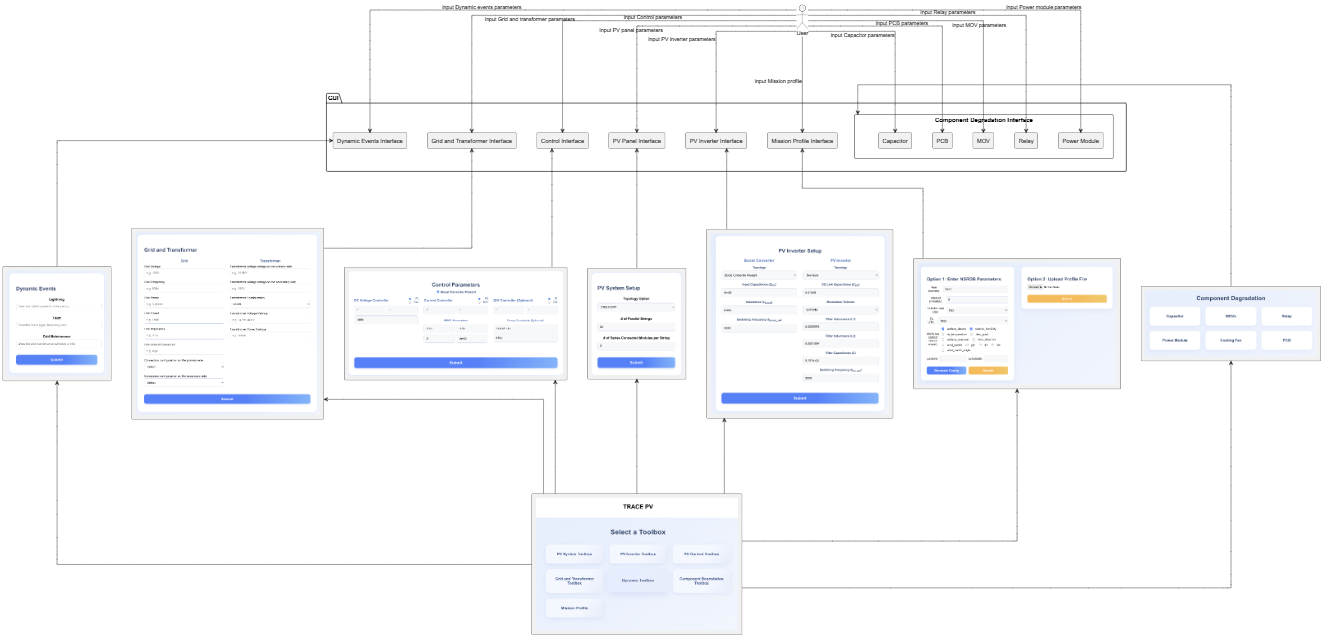
\includegraphics[width=\textwidth]{figure2.png}
    \caption{GUI Dataflow}
\end{figure}

\begin{figure}[h]
    \centering
    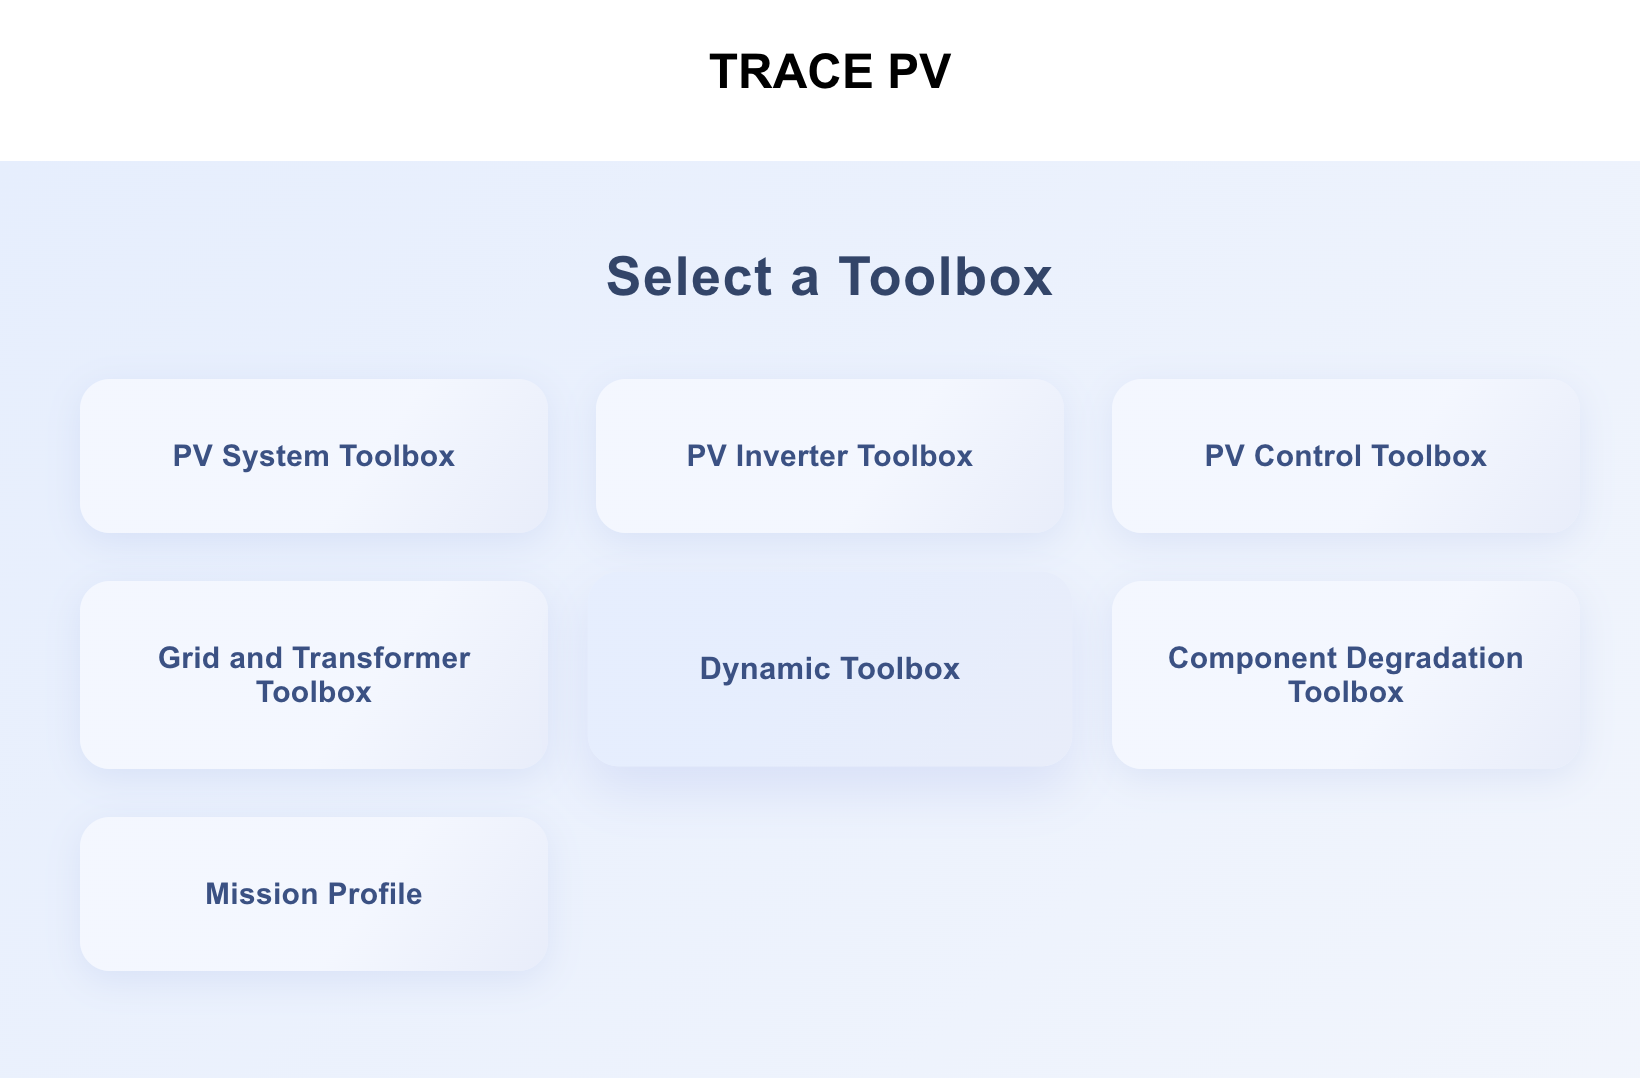
\includegraphics[width=\textwidth]{figure3.png}
    \caption{GUI Overview}
\end{figure}

\subsection{Mission Profile}
The Mission profile interface is shown in Figure 4. For mission profile, the TRACE-PV tools require two types of mission profiles: environmental condition and the operating condition. There are two options: 1. NSRDB; 2. User input.

\begin{figure}[h]
    \centering
    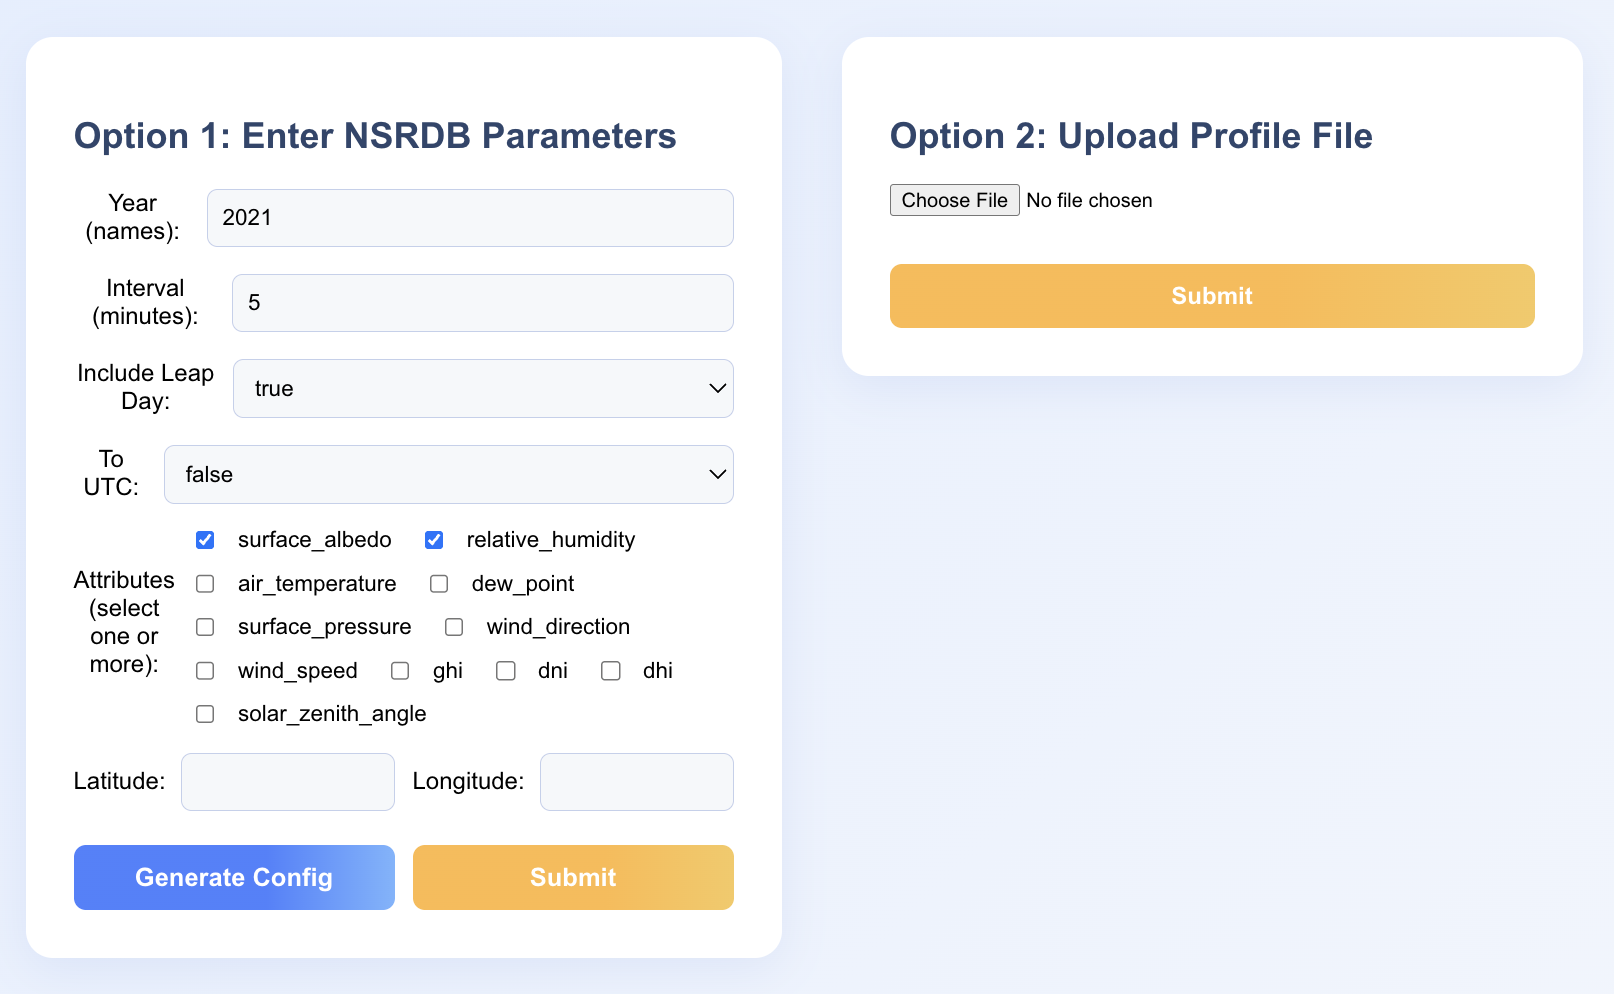
\includegraphics[width=\textwidth]{figure4.png}
    \caption{Mission Profile Interface}
\end{figure}

\subsubsection{Mission Profile User Input}
\paragraph{Environmental Condition User Input}
Users will provide environmental conditions by uploading files to the GUI. Only comma-separated values (CSV) file is supported. The file to be uploaded needs to include operating conditions (three data fields: AC voltage, power ratio) and environmental condition (three fields: solar irradiance, ambient temperature, relative humidity). Details are listed in Table 1. The environmental condition can also be provided via 1.1.2 Mission Profile Database (NRSDB).

\begin{table}[h]
\centering
\caption{Mission Profile Class (Environmental Condition)}
\begin{tabular}{|l|p{3cm}|l|l|p{6cm}|}
\hline
\textbf{No.} & \textbf{Variable Name} & \textbf{Data Type} & \textbf{Unit} & \textbf{Description} \\ \hline
1 & Latitude & Float & $^\circ$ & Latitude of the target location \\ \hline
2 & Longitude & Float & $^\circ$ & Longitude of the target location \\ \hline
3 & Year & integer & N/A & Calendar year of the record \\ \hline
4 & IR & Float[] & W/m$^2$ & Solar Irradiance (Environmental Condition) \\ \hline
5 & Tamb & Float[] & $^\circ$F & Ambient Temperature (Environmental Condition) \\ \hline
6 & RH & Float[] & \% & Relative Humidity (Environmental Condition) \\ \hline
\end{tabular}
\end{table}

\paragraph{Grid Operating Condition User Input}

\begin{table}[h]
\centering
\caption{Mission Profile Class (Grid Operating Condition)}
\begin{tabular}{|l|l|l|l|p{6cm}|}
\hline
\textbf{No.} & \textbf{Variable Name} & \textbf{Data Type} & \textbf{Unit} & \textbf{Description} \\ \hline
1 & Vac & Float[] & V & AC Voltage (Operating Condition) \\ \hline
2 & PF & Float[] & N/A & Power Factor (Operating Condition) \\ \hline
\end{tabular}
\end{table}

\subsubsection{Mission Profile Database (NRSDB)}
By leveraging the API of NSRDB, the environment conditions can be retrieved via providing the location information (latitude \& longitude); time series information (year, time resolution). Grid operating conditions require user inputs.

\begin{table}[h]
\centering
\caption{NRSDB}
\begin{tabular}{|l|l|l|l|p{6cm}|}
\hline
\textbf{No.} & \textbf{Variable Name} & \textbf{Data Type} & \textbf{Unit} & \textbf{Description} \\ \hline
\multicolumn{5}{|l|}{\textbf{Primary keys}} \\ \hline
1 & Latitude & Float & $^\circ$ & Latitude of the target location \\ \hline
2 & Longitude & Float & $^\circ$ & Longitude of the target location \\ \hline
3 & Year & integer & N/A & Calendar year of the record \\ \hline
4 & Interval & Integer & N/A & Time resolution of the record \\ \hline
\multicolumn{5}{|l|}{\textbf{Dependent Attributes}} \\ \hline
5 & IR & Float[] & W/m$^2$ & Solar Irradiance (Environmental Condition) \\ \hline
6 & Tamb & Float[] & $^\circ$F & Ambient Temperature (Environmental Condition) \\ \hline
7 & RH & Float[] & \% & Relative Humidity (Environmental Condition) \\ \hline
\end{tabular}
\end{table}

Note that locations within the U.S. support up to 1-minute intervals, while locations outside the U.S. support 10-minute intervals. If the data for the location is not available in NRSDB, user has to choose option 2 to upload the environmental conditions. Only environmental conditions are available in NRSDB.

\subsection{PV System}
The PV system interface is shown in Figure 5. It takes the user input of the PV module part number and corresponding grid configuration, saved in PVSystem class, as shown in Table 4. And for each PV module part, an offline database is established. Details are shown in Table 7.

\begin{figure}[h]
    \centering
    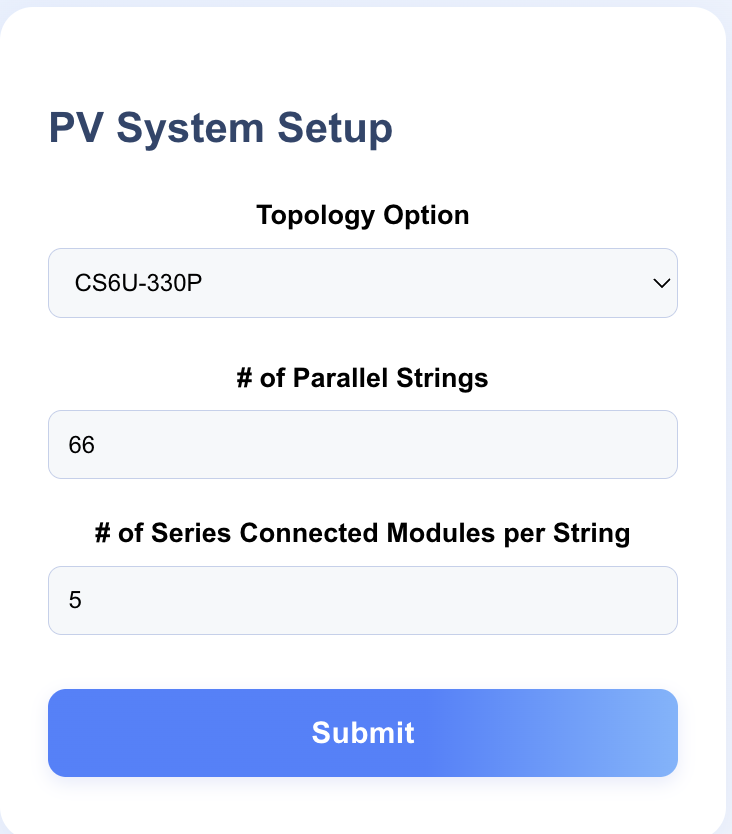
\includegraphics[width=\textwidth]{figure5.png}
    \caption{PV System Interface}
\end{figure}

\begin{figure}[h]
    \centering
    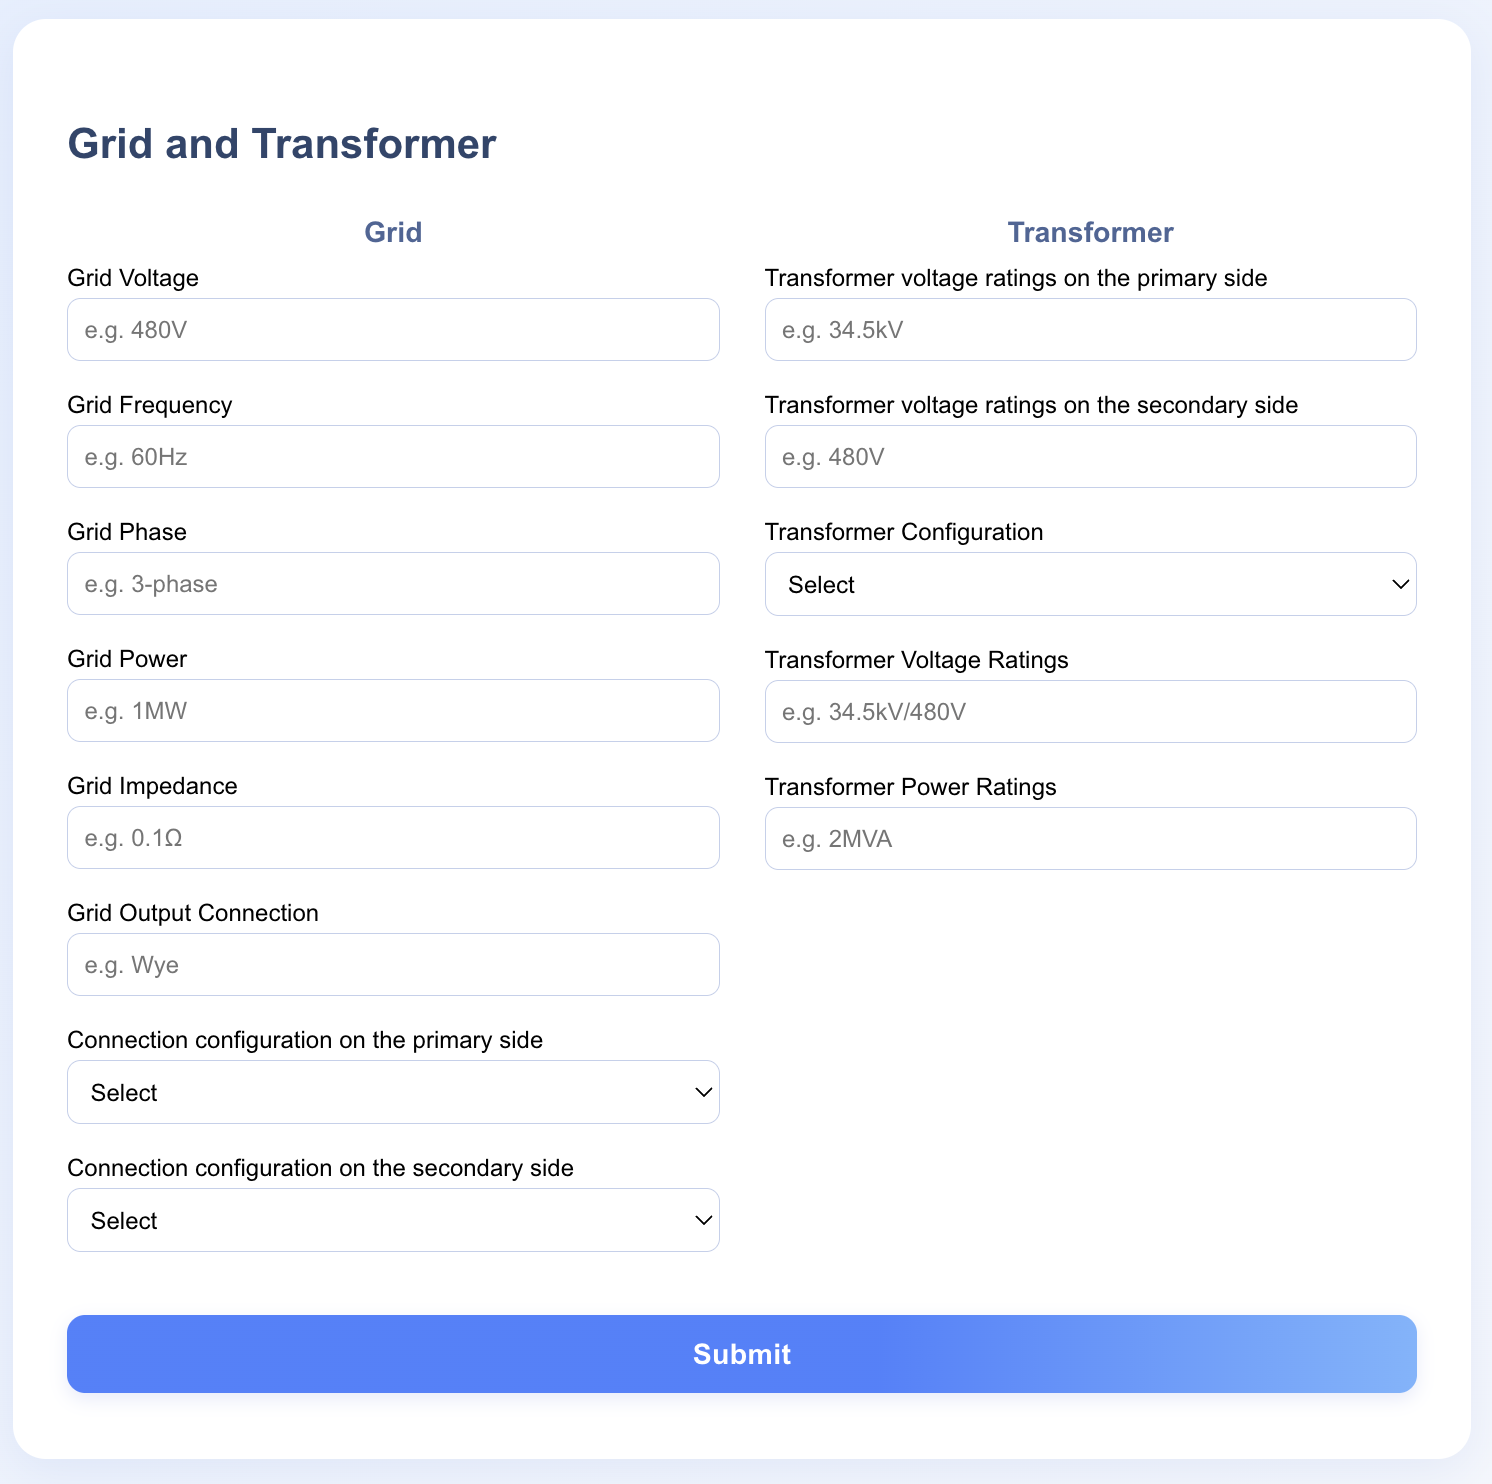
\includegraphics[width=\textwidth]{figure6.png}
    \caption{Grid and Transformer Interface}
\end{figure}

\subsubsection{PV System User Input}
PV System class includes PV module part number and corresponding configuration. Besides, the configuration of the grid connected to the PV system is also included.

\paragraph{PV Module User Input}
\begin{table}[h]
\centering
\caption{PV System Class (PV Module)}
\begin{tabular}{|l|p{3cm}|l|l|p{6cm}|}
\hline
\textbf{No.} & \textbf{Variable Name} & \textbf{Data Type} & \textbf{Unit} & \textbf{Description} \\ \hline
1 & pvModulePartNumber & Enum & N/A & part number of the PV module used in the PV system. \\ \hline
2 & numberOfParallelStrings & Integer & N/A & Number of parallel-connected PV strings in the array, defining the total current capability. \\ \hline
3 & numberOfSeries & Integer & N/A & Number of series-connected modules in each string, defining the total voltage capability. \\ \hline
\end{tabular}
\end{table}

\paragraph{Transformer User Input}
\begin{table}[h]
\centering
\caption{PV System Class (Transformer)}
\begin{tabular}{|l|p{4cm}|l|l|p{5cm}|}
\hline
\textbf{No.} & \textbf{Variable Name} & \textbf{Data Type} & \textbf{Unit} & \textbf{Description} \\ \hline
1 & transformerPrimaryVoltage & Float & kV & The voltage rating for the primary side of the transformer. \\ \hline
2 & transformerSecondaryVoltage & Float & V & The voltage rating for the secondary side of the transformer. \\ \hline
3 & transformerConfiguration & Enum & N/A & The winding configuration of the transformer \\ \hline
4 & transformerPowerRatings & Float & MVA & The power rating of the transformer \\ \hline
\end{tabular}
\end{table}

\paragraph{Grid User Input}
\begin{table}[h]
\centering
\caption{PV System Class (Grid)}
\begin{tabular}{|l|l|l|l|p{6cm}|}
\hline
\textbf{No.} & \textbf{Variable Name} & \textbf{Data Type} & \textbf{Unit} & \textbf{Description} \\ \hline
1 & gridVoltage & Float & V & Nominal RMS line-to-line (or phase-to-phase) voltage of the connected AC grid. \\ \hline
2 & gridFrequency & Float & Hz & Nominal operating frequency of the AC grid, typically 50 Hz or 60 Hz. \\ \hline
3 & gridImpedance & Float & $\Omega$ & Equivalent grid impedance (resistance and reactance) as seen from the inverter connection point. \\ \hline
\end{tabular}
\end{table}

\subsubsection{PV System Database}
The PV module database includes the IV curve and output voltage under different combinations of temperature and solar irradiance conditions for each model PV module.

\begin{table}[h]
\centering
\caption{PV Module Database}
\begin{tabular}{|l|p{3cm}|l|l|p{6cm}|}
\hline
\textbf{No.} & \textbf{Variable Name} & \textbf{Data Type} & \textbf{Unit} & \textbf{Description} \\ \hline
\multicolumn{5}{|l|}{\textbf{Primary Key}} \\ \hline
1 & pvModulePartNumber & Enum & N/A & Identification code or part number of the PV module used in the system. \\ \hline
2 & IR & float & W/m$^2$ & I–V curves of the PV module under varying irradiance and temperature conditions. \\ \hline
3 & Temp & float & $^\circ$F & Output voltage of the PV module. \\ \hline
4 & numberOfParallelStrings & Integer & N/A & Number of parallel-connected PV strings in the array, defining the total current capability. \\ \hline
5 & numberOfSeries & Integer & N/A & Number of series-connected modules in each string, defining the total voltage capability. \\ \hline
\multicolumn{5}{|l|}{\textbf{Dependent Attributes}} \\ \hline
1 & IvCurve & float[] & A/V & I–V curves of the PV module under varying irradiance and temperature conditions. \\ \hline
\end{tabular}
\end{table}

\subsection{PV Inverter}
\subsubsection{PV Inverter User Input}
\begin{figure}[h]
    \centering
    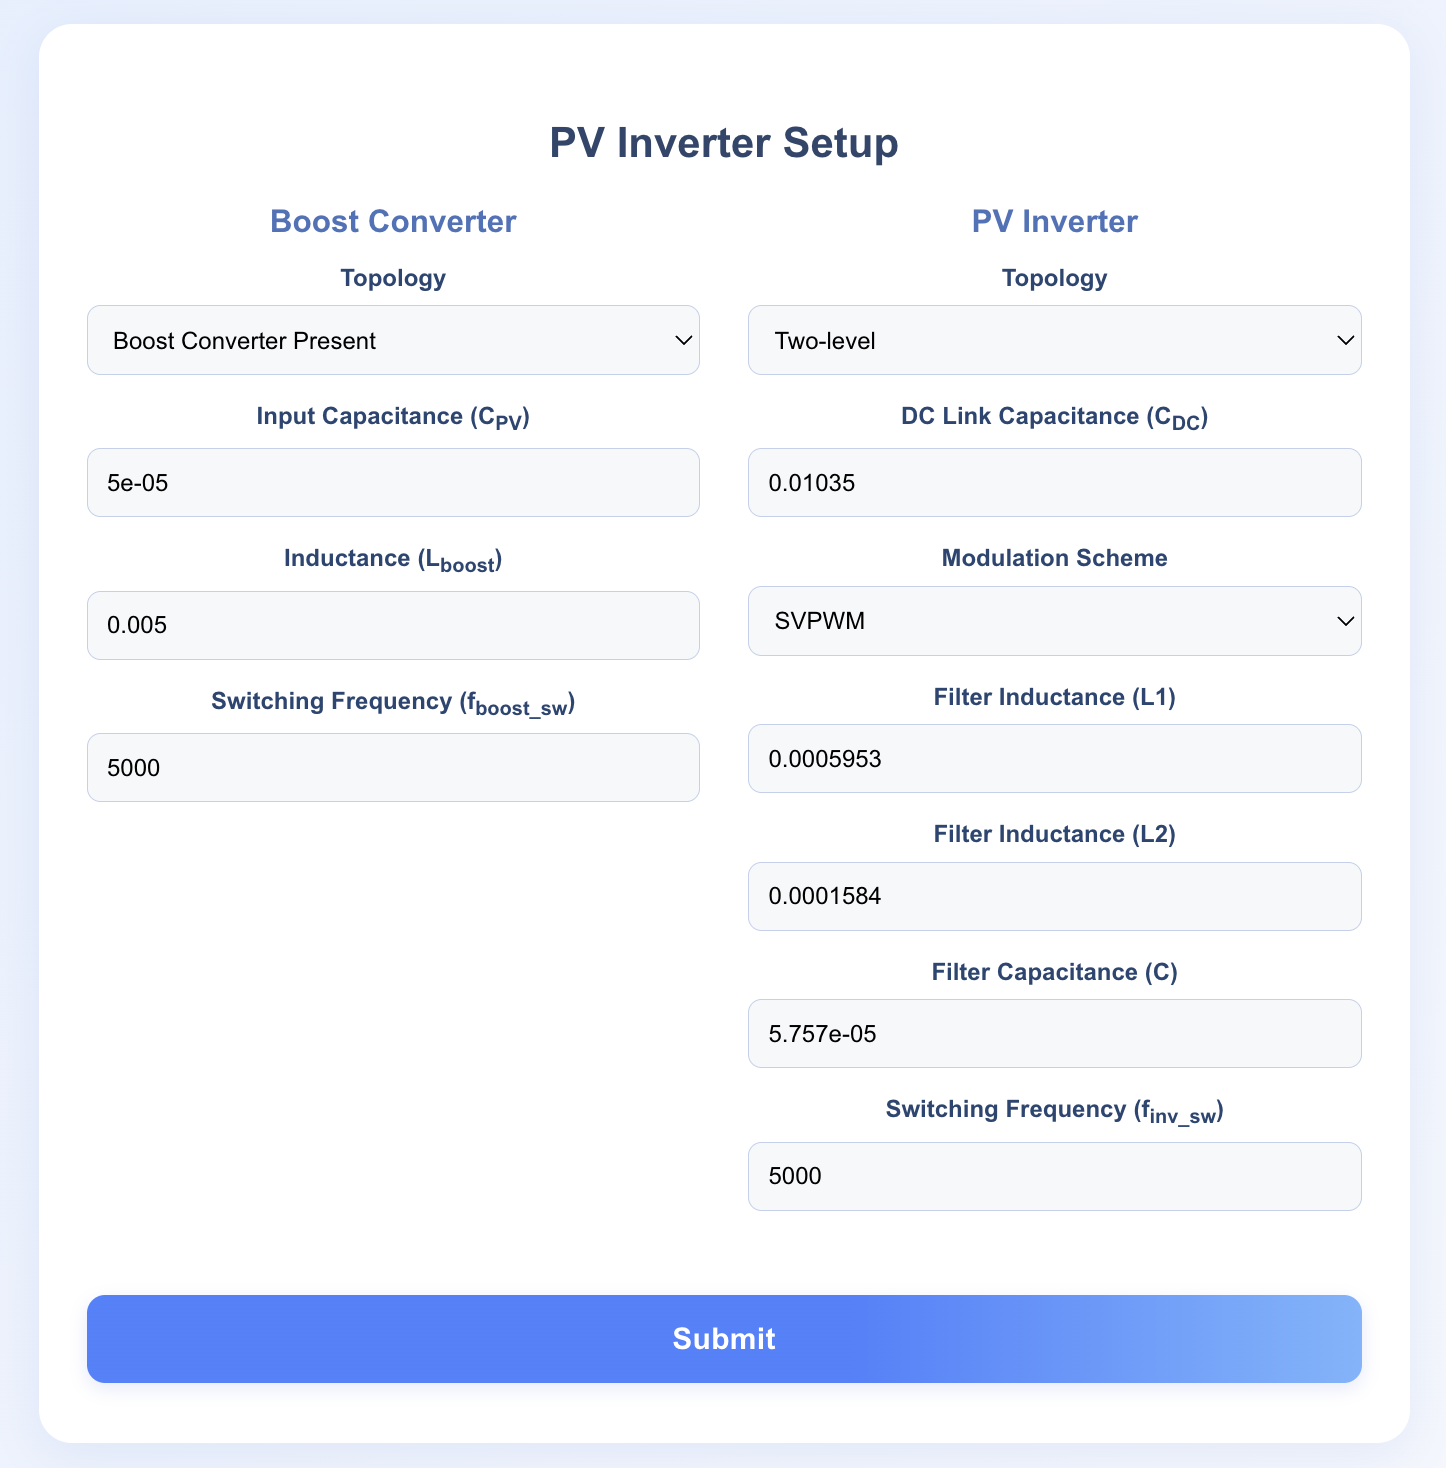
\includegraphics[width=\textwidth]{figure7.png}
    \caption{PV Inverter Interface}
\end{figure}

PV inverter class considers two topologies: whether the boost converter present or not. And includes the part number of each PV inverter. Details are shown in Table 8.

\begin{table}[h]
\centering
\caption{PV Inverter Class}
\begin{tabular}{|l|p{4cm}|l|l|p{5cm}|}
\hline
\textbf{No.} & \textbf{Variable Name} & \textbf{Data Type} & \textbf{Unit} & \textbf{Description} \\ \hline
1 & pvInverterConfiguration & Boolean & N/A & Specifies whether a boost converter stage is included in the inverter. \\ \hline
\multicolumn{5}{|l|}{\textbf{Inverter related parameters}} \\ \hline
2 & pvInverterPartNumber & Enum & N/A & Identification code or part number of the PV inverter. \\ \hline
3 & pvInverterTopology & Enum & N/A & Inverter topology type, [`Two-level', `NPC', `ANPC', `T-type']. \\ \hline
4 & inverterModulationScheme & Enum & N/A & Inverter modulation method, [`PWM', `SPWM']. \\ \hline
5 & inverterSwitchingFrequency & Float & Hz & Switching frequency of the boost converter. \\ \hline
6 & CDC & Float & F & DC-link capacitance \\ \hline
7 & L1 & Float & H & Converter-side inductor \\ \hline
8 & R1 & Float & $\Omega$ & Converter-side resistance \\ \hline
9 & C & Float & F & Filter capacitor \\ \hline
10 & L2 & Float & H & Grid-side inductor \\ \hline
11 & R2 & Float & $\Omega$ & Grid-side resistance \\ \hline
\multicolumn{5}{|l|}{\textbf{Boost Converter (Optional)}} \\ \hline
12 & boostCapacitance & Float & F & Capacitance of the boost converter. \\ \hline
13 & boostInductance & Float & H & Inductance of the boost converter. \\ \hline
14 & boostResistance & Float & $\Omega$ & Series resistance of the boost converter inductor. \\ \hline
15 & boostSwitchingFrequency & Float & Hz & Switching frequency of the boost converter. \\ \hline
\end{tabular}
\end{table}

\subsubsection{PV Inverter Database}
PV inverter database includes the capacitance, modulation scheme and inductance value for each PV inverter model. Details are shown in This information can be retrieved according to the PV inverter part number and modulation scheme.

\begin{table}[h]
\centering
\caption{PV Inverter Database}
\begin{tabular}{|l|p{3.5cm}|l|l|p{5.5cm}|}
\hline
\textbf{No.} & \textbf{Variable Name} & \textbf{Data Type} & \textbf{Unit} & \textbf{Description} \\ \hline
\multicolumn{5}{|l|}{\textbf{Primary Keys}} \\ \hline
1 & pvInverterConfiguration & Boolean & N/A & Specifies whether a boost converter stage is included in the inverter. \\ \hline
2 & pvInverterTopology & Enum & N/A & Inverter topology type, [`Two-level', `NPC', `ANPC', `T-type']. \\ \hline
\multicolumn{5}{|l|}{\textbf{Dependent Attributes}} \\ \hline
3 & avgOde & Float[] & 2.1.4 & Average model ODE \\ \hline
4 & swODE & Float[] & 2.1.3 & Switching model ODE \\ \hline
\end{tabular}
\end{table}

\textbf{avgODE:}\\
Single-stage two-level\\
Two-stage two-level\\
Single-stage three-level\\
Two-stage three-level\\

\textbf{swODE:}\\
Single-stage two-level\\
Two-stage two-level\\
Single-stage three-level\\
Two-stage three-level

\subsubsection{Modulation scheme database}
\begin{table}[h]
\centering
\caption{Modulation Database}
\begin{tabular}{|l|l|l|l|p{6cm}|}
\hline
\textbf{No.} & \textbf{Variable Name} & \textbf{Data Type} & \textbf{Unit} & \textbf{Description} \\ \hline
\multicolumn{5}{|l|}{\textbf{Primary Keys}} \\ \hline
1 & inverterModulationScheme & Enum & N/A & Inverter modulation method, [`SPWM', `SVM']. \\ \hline
2 & inverterSwitchingFrequency & Float & Hz & Switching frequency of the boost converter. \\ \hline
3 & da & Float[] & N/A & Duty ratio of phase A leg \\ \hline
4 & db & Float[] & N/A & Duty ratio of phase B leg \\ \hline
5 & dc & Float[] & N/A & Duty ratio of phase C leg \\ \hline
\multicolumn{5}{|l|}{\textbf{Dependent Attributes}} \\ \hline
3 & Sa\_T & Float[] & N/A & Switching state function for the phase A leg vs. Time \\ \hline
4 & Sb\_T & Float[] & N/A & Switching state function for the phase B leg vs. Time \\ \hline
 & Sc\_T & Float[] & N/A & Switching state function for the phase C leg vs. Time \\ \hline
\end{tabular}
\end{table}

Two cases: SPWM, SVM [`various variation']

\subsection{Control}
\begin{figure}[h]
    \centering
    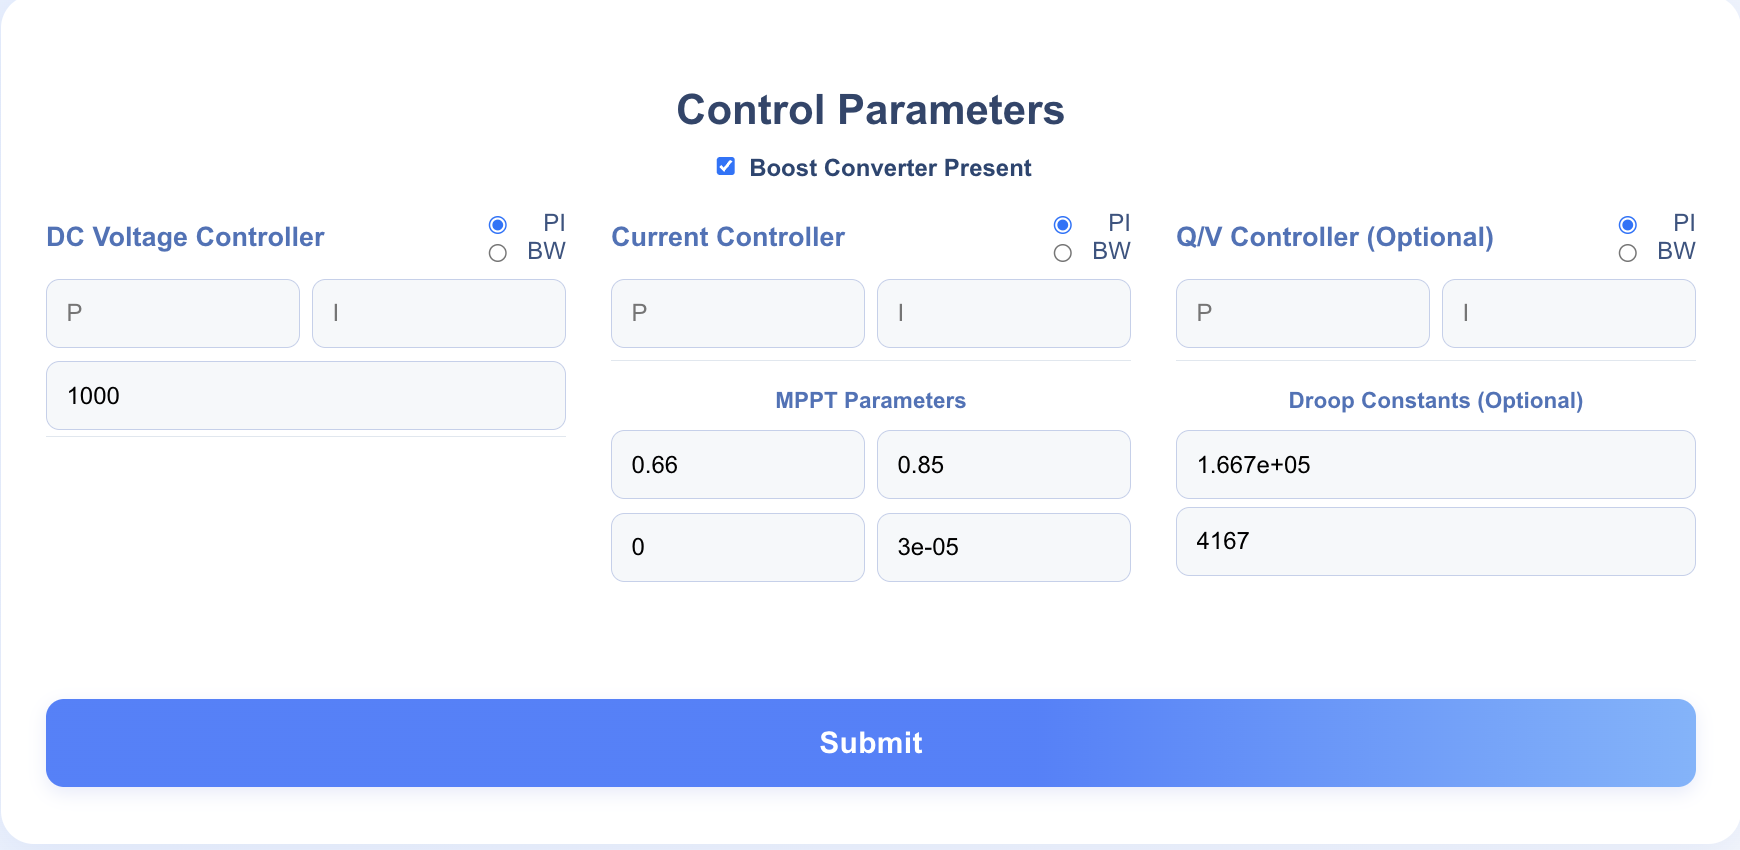
\includegraphics[width=\textwidth]{figure8.png}
    \caption{Control Interface}
\end{figure}

\subsubsection{Control User Input}
Control class includes the control strategy and the corresponding parameters, as shown in Table 11.

\begin{table}[h]
\centering
\caption{Control Class}
\begin{tabular}{|l|l|l|l|p{6cm}|}
\hline
\textbf{No.} & \textbf{Variable Name} & \textbf{Data Type} & \textbf{Unit} & \textbf{Description} \\ \hline
1 & controlStrategy & Enum & N/A & Control parameter database for the PV inverter. Eg. Open loop, close loop (traditional, advanced) \\ \hline
\end{tabular}
\end{table}

\subsubsection{Control Database}
Control database includes control parameters, which can be retrieved via the control strategy. Details are shown in Table 12.

\begin{table}[h]
\centering
\caption{Control Database Class}
\begin{tabular}{|l|l|l|l|p{6cm}|}
\hline
\textbf{No.} & \textbf{Variable Name} & \textbf{Data Type} & \textbf{Unit} & \textbf{Description} \\ \hline
\multicolumn{5}{|l|}{\textbf{Primary Key}} \\ \hline
1 & controlStrategy & Enum & N/A & Control parameter database for the PV inverter. (Open loop) \\ \hline
\multicolumn{5}{|l|}{\textbf{Dependent Attributes}} \\ \hline
2 & da & Float[] & N/A & Duty ratio of phase A leg \\ \hline
3 & db & Float[] & N/A & Duty ratio of phase B leg \\ \hline
4 & dc & Float[] & N/A & Duty ratio of phase C leg \\ \hline
\end{tabular}
\end{table}

\textbf{Open loop:}
\begin{equation}
da = \frac{1+M_I \cdot \sin(\omega \cdot t)}{2}
\end{equation}
\begin{equation}
db = \frac{1+M_I \cdot \sin(\omega \cdot t - \frac{2\pi}{3})}{2}
\end{equation}
\begin{equation}
dc = \frac{1+M_I \cdot \sin(\omega \cdot t - \frac{4\pi}{3})}{2}
\end{equation}

\textbf{Closed loop:} Traditional, Advanced

\subsection{Dynamic Events}
\begin{figure}[h]
    \centering
    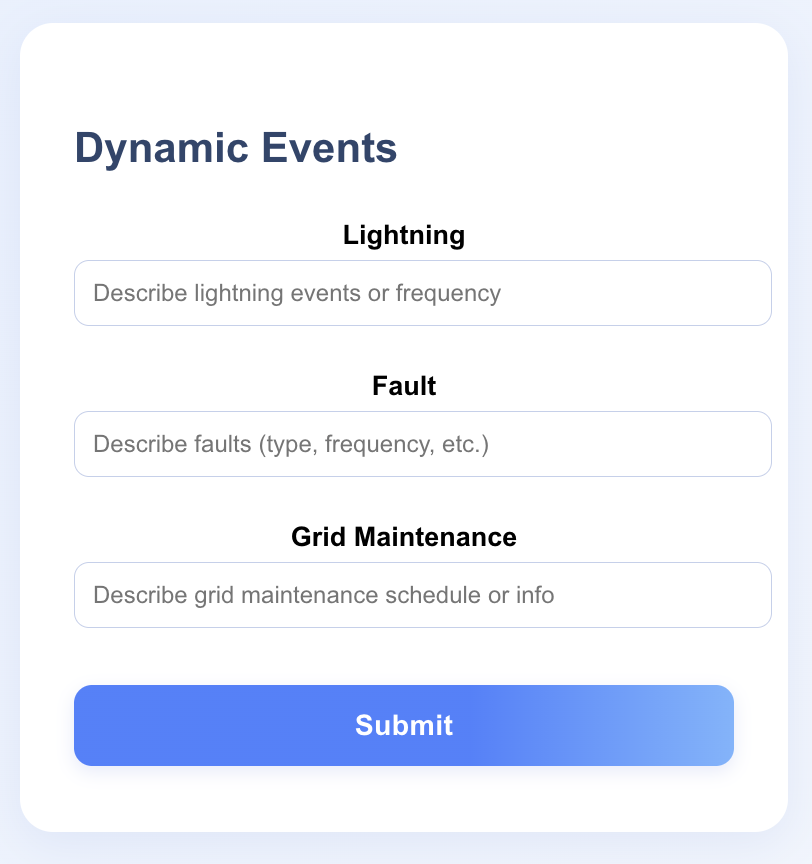
\includegraphics[width=\textwidth]{figure9.png}
    \caption{Dynamic Events Interface}
\end{figure}

\subsubsection{Dynamic Events User Input}
Dynamic events class includes the event type, happened time and duration

\begin{table}[h]
\centering
\caption{DynamicEvents Class}
\begin{tabular}{|l|l|l|p{6cm}|}
\hline
\textbf{Variable Name} & \textbf{Data Type} & \textbf{Unit} & \textbf{Description} \\ \hline
Latitude & Float & $^\circ$ & Latitude of the target location \\ \hline
Longitude & Float & $^\circ$ & Longitude of the target location \\ \hline
eventID & integer & N/A & The event ID of the dynamic event \\ \hline
\end{tabular}
\end{table}

\subsubsection{Dynamic Events Database}
The dynamic event database includes the dynamic events with details and can be queried via the location information and eventID.

\begin{table}[h]
\centering
\caption{DynamicEventsDB Class}
\begin{tabular}{|l|l|l|p{6cm}|}
\hline
\textbf{Variable Name} & \textbf{Data Type} & \textbf{Unit} & \textbf{Description} \\ \hline
Latitude & Float & $^\circ$ & Latitude of the target location \\ \hline
Longitude & Float & $^\circ$ & Longitude of the target location \\ \hline
eventID & Integer & N/A & \\ \hline
eventType & Enum & N/A & Category or type of the dynamic event. \\ \hline
eventTime & Datatime & s & Timestamp indicating when the event occurs. \\ \hline
eventDuration & float & s & Time span for which the event lasts. \\ \hline
\end{tabular}
\end{table}

\subsection{Component Degradation}
\begin{figure}[h]
    \centering
    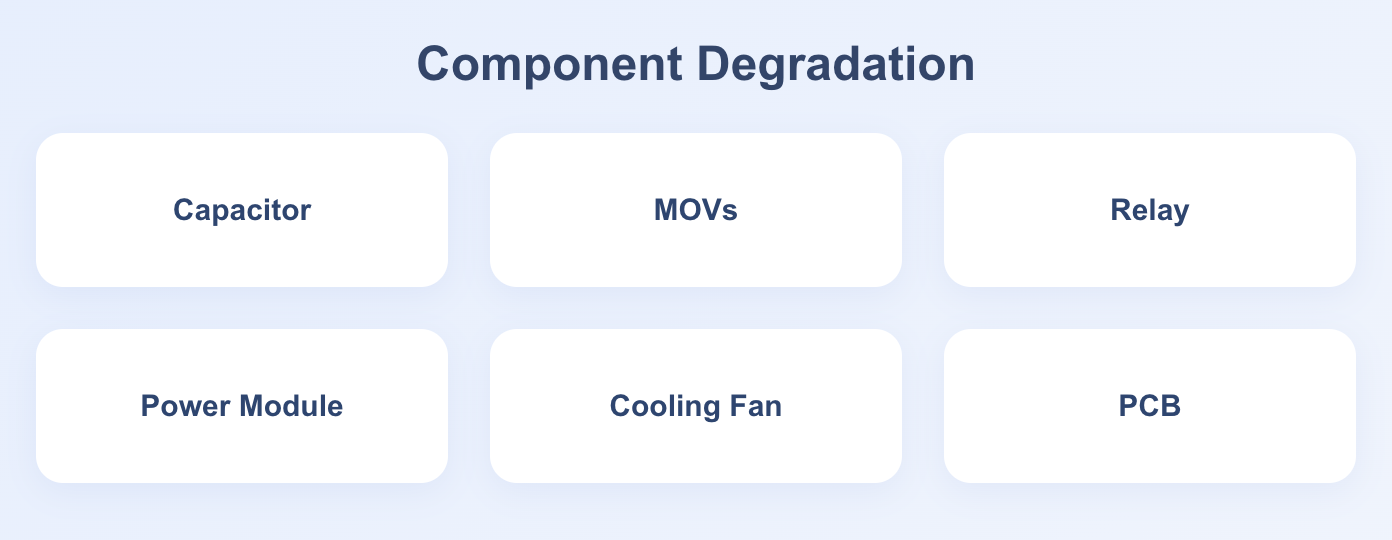
\includegraphics[width=\textwidth]{figure10.png}
    \caption{Component Degradation Interface}
\end{figure}

\subsubsection{Power Module}
Power module class includes the part number of the power module. And the corresponding database includes ESR and RTH of each model.

\paragraph{Power Module User Input}
\begin{table}[h]
\centering
\caption{Power Module Class}
\begin{tabular}{|l|l|l|l|p{6cm}|}
\hline
\textbf{No.} & \textbf{Variable Name} & \textbf{Data Type} & \textbf{Unit} & \textbf{Description} \\ \hline
1 & pmPartNumber & String & N/A & Identification code or manufacturer part number of the power module. \\ \hline
\end{tabular}
\end{table}

\paragraph{Power Module Database}
\begin{table}[h]
\centering
\caption{Power Module Database}
\begin{tabular}{|l|l|l|l|p{6cm}|}
\hline
\textbf{No.} & \textbf{Variable Name} & \textbf{Data Type} & \textbf{Unit} & \textbf{Description} \\ \hline
\multicolumn{5}{|l|}{\textbf{Primary Key}} \\ \hline
1 & pmPartNumber & Enum & N/A & Manufacturer part number of the power module. \\ \hline
\multicolumn{5}{|l|}{\textbf{Dependent Attributes}} \\ \hline
2 & rth & float & $^\circ$C/W & Thermal resistance of the power module. \\ \hline
3 & Von\_Ic\_Tj & Float[] & V & On-State Voltage vs. Collector current and temperature \\ \hline
4 & Eon\_Ic\_Vce\_Tj & Float[] & J & The turn-on energy loss vs. inductor current and the blocking voltage \\ \hline
5 & Eoff\_Ic\_Vce\_Tj & Float[] & J & The turn-off energy loss vs. Inductor current and the blocking voltage \\ \hline
6 & ERR\_Ic\_Vce\_Tj & Float[] & J & Reverse recovery energy loss vs. inductor current and the block voltage \\ \hline
7 & PM\_reliability\_coef\_thermal & Float[] & N/A & Reliability model coefficients for power module thermal model include A, n and Ea \\ \hline
8 & PM\_reliability\_coef\_RH & Float[] & N/A & Reliability model coefficients for power module RH model include n1, n2 \\ \hline
\end{tabular}
\end{table}

Power module thermal reliability model:
\begin{equation}
N_f = A \times \Delta T^n \times e^{\frac{E_a}{K_B T_{max}}}
\end{equation}

Power module RH reliability model:
\begin{equation}
\text{Lifetime} = \text{Lifetime}_{stress} \cdot \left(\frac{RH_{stress}}{RH_{op}}\right)^{n1} \cdot \exp\left(\frac{E_a}{k_B} \cdot \left(\frac{1}{T_{op}} - \frac{1}{T_{stress}}\right)\right) \cdot \left(\frac{Voltage_{stress}}{Voltage_{op}}\right)^{n2}
\end{equation}

\subsubsection{Capacitor}
\paragraph{Capacitor User Input}
\begin{table}[h]
\centering
\caption{Capacitor Class}
\begin{tabular}{|l|l|l|l|p{6cm}|}
\hline
\textbf{No.} & \textbf{Variable Name} & \textbf{Data Type} & \textbf{Unit} & \textbf{Description} \\ \hline
1 & capType & Enum & N/A & The type of capacitor \\ \hline
2 & capPartNumber & Enum & N/A & Identification code or manufacturer part number of the power module. \\ \hline
\end{tabular}
\end{table}

\paragraph{Capacitor Database}
\begin{table}[h]
\centering
\caption{Capacitor Database}
\begin{tabular}{|l|l|l|l|p{6cm}|}
\hline
\textbf{No.} & \textbf{Variable Name} & \textbf{Data Type} & \textbf{Unit} & \textbf{Description} \\ \hline
\multicolumn{5}{|l|}{\textbf{Primary Key}} \\ \hline
1 & capPartNumber & Enum & N/A & Identification code or manufacturer part number of the power module. \\ \hline
2 & capType & Enum & N/A & The type of capacitor \\ \hline
\multicolumn{5}{|l|}{\textbf{Dependent Attributes}} \\ \hline
3 & Capacitance\_T\_V & Float[] & F & Capacitance value of the capacitor vs. Temperature and voltage \\ \hline
4 & Esr\_T\_freq & Float[] & J & Energy dissipated during diode reverse recovery vs. Temperature and frequency \\ \hline
5 & Rth\_ah & Float[] & $^\circ$C/W & Thermal resistance from ambient to hotspot \\ \hline
6 & Rth\_as & Float[] & $^\circ$C/W & Thermal resistance from ambient to surface \\ \hline
7 & Cap\_freq? & integer & Hz & DC-link capacitor frequency \\ \hline
8 & Cap\_reliability\_coef & Float[] & N/A & Capacitor reliability model coefficients include A, n, Ea, $\beta$ for film capacitor \\ \hline
\end{tabular}
\end{table}

Film capacitor reliability model:
\begin{equation}
\text{Lifetime} = A \cdot (RH_{op})^{-n} \cdot \exp\left(\frac{E_a}{k_B} \cdot \frac{1}{T_{op}}\right) \cdot \exp(\beta \cdot V_{op})
\end{equation}

Electrolytic reliability model:
\begin{equation}
\text{Lifetime} = L_0 \cdot \left(\frac{V}{V_0}\right)^{-\beta_1} \cdot 2^{\frac{T_0 - T_1}{10}}
\end{equation}

\subsubsection{PCB}
\paragraph{PCB User Input}
\begin{table}[h]
\centering
\caption{PCB Class}
\begin{tabular}{|l|l|l|l|p{6cm}|}
\hline
\textbf{No.} & \textbf{Variable Name} & \textbf{Data Type} & \textbf{Unit} & \textbf{Description} \\ \hline
1 & footprint & Enum & N/A & The footprint soldered on the PCB: [`Decoupling', `MELF'] \\ \hline
2 & solderJoint material & Enum & N/A & The material of the solder joint, eg. Leaded SnPb, Leadless SAC \\ \hline
3 & Thickness & Float & mm & The thickness of PCB \\ \hline
4 & Dimensions & float[] & mm & Physical dimensions of the PCB (component, copper pad, solder joint) \\ \hline
\end{tabular}
\end{table}

\paragraph{PCB Database}
\begin{table}[h]
\centering
\caption{PCB Database}
\begin{tabular}{|l|l|l|l|p{6cm}|}
\hline
\textbf{No.} & \textbf{Variable Name} & \textbf{Data Type} & \textbf{Unit} & \textbf{Description} \\ \hline
\multicolumn{5}{|l|}{\textbf{Primary Keys}} \\ \hline
1 & footprint & Enum & N/A & The footprint soldered on the PCB: [`Decoupling', `MELF'] \\ \hline
2 & solderJoint material & Enum & N/A & The material of the solder joint, eg. Leaded SnPb, Leadless SAC \\ \hline
3 & Thickness & Float & mm & The thickness of PCB \\ \hline
4 & Dimensions & float[] & mm & Physical dimensions of the PCB (component, copper pad, solder joint) \\ \hline
\multicolumn{5}{|l|}{\textbf{Dependent Attributes}} \\ \hline
1 & PCB\_reliability\_coef & float[] & N/A & PCB Reliability coefficients \\ \hline
\end{tabular}
\end{table}

PCB Reliability Model:
\begin{equation}
N_{f,50\%} = \left(\frac{\Delta W}{\epsilon_f}\right)^{c_{fatigue}}
\end{equation}
\begin{equation}
\Delta W = C \cdot \tau \cdot \Delta \gamma
\end{equation}
\begin{equation}
\tau = K(\alpha_b - \alpha_c)\Delta T \frac{L_d}{A}
\end{equation}
\begin{equation}
\Delta \gamma = 1.383 \frac{L_d^3}{A h} (\alpha_c \Delta T_c - \alpha_b \Delta T_b)
\end{equation}

\subsubsection{Cooling Fan}
\paragraph{Cooling Fan Input}
\begin{table}[h]
\centering
\caption{Cooling Fan Class}
\begin{tabular}{|l|l|l|l|p{6cm}|}
\hline
\textbf{No.} & \textbf{Variable Name} & \textbf{Data Type} & \textbf{Unit} & \textbf{Description} \\ \hline
1 & coolingFanPartNumber & Enum & N/A & Manufacturer part number of the Cooling Fan \\ \hline
\end{tabular}
\end{table}

\paragraph{Cooling Fan Database}
\begin{table}[h]
\centering
\caption{Cooling Fan Database}
\begin{tabular}{|l|l|l|l|p{6cm}|}
\hline
\textbf{No.} & \textbf{Variable Name} & \textbf{Data Type} & \textbf{Unit} & \textbf{Description} \\ \hline
\multicolumn{5}{|l|}{\textbf{Primary Key}} \\ \hline
1 & coolingFanPartNumber & Enum & N/A & Manufacturer part number of the Cooling Fan \\ \hline
\multicolumn{5}{|l|}{\textbf{Dependent Attributes}} \\ \hline
2 & CoolingFan\_reliability\_coef\_mechanical & float[] & N/A & Cooling fan reliability model coefficient considering mechanical failure \\ \hline
3 & CoolingFan\_reliability\_coef\_electrical & float[] & N/A & Cooling fan reliability model coefficient considering electrical failure \\ \hline
\end{tabular}
\end{table}

\subsubsection{MOV}
\paragraph{MOV User Input}
\begin{table}[h]
\centering
\caption{MOV Class}
\begin{tabular}{|l|l|l|l|p{6cm}|}
\hline
\textbf{No.} & \textbf{Variable Name} & \textbf{Data Type} & \textbf{Unit} & \textbf{Description} \\ \hline
1 & movPartNumber & Enum & N/A & Identification code or manufacturer part number of the MOV \\ \hline
\end{tabular}
\end{table}

\paragraph{MOV Database}
\begin{table}[h]
\centering
\caption{MOV Database}
\begin{tabular}{|l|l|l|l|p{6cm}|}
\hline
\textbf{No.} & \textbf{Variable Name} & \textbf{Data Type} & \textbf{Unit} & \textbf{Description} \\ \hline
1 & movPartNumber (Primary Key) & Enum & N/A & Identification code or manufacturer part number of the MOV \\ \hline
2 & ivCurve & float[] & V/A & Current–voltage characteristic curve of the device. \\ \hline
3 & pulseRatingCurve & float[] & Stress vs. cycles & Lifetime curve of the device under electrical cycling stress. \\ \hline
\end{tabular}
\end{table}

\subsubsection{Relay}
\paragraph{Relay User Input}
\begin{table}[h]
\centering
\caption{Relay Class}
\begin{tabular}{|l|l|l|l|p{6cm}|}
\hline
\textbf{No.} & \textbf{Variable Name} & \textbf{Data Type} & \textbf{Unit} & \textbf{Description} \\ \hline
1 & relayPartNumber & Enum & N/A & Identification code or manufacturer part number of the Relay \\ \hline
\end{tabular}
\end{table}

\paragraph{Relay Database}
\begin{table}[h]
\centering
\caption{Relay Database}
\begin{tabular}{|l|l|l|l|p{6cm}|}
\hline
\textbf{No.} & \textbf{Variable Name} & \textbf{Data Type} & \textbf{Unit} & \textbf{Description} \\ \hline
1 & relayPartNumber (Primary Key) & Enum & N/A & Identification code or manufacturer part number of the Relay \\ \hline
2 & ivCurve & float[] & V/A & Current–voltage characteristic curve of the device. \\ \hline
3 & electricalLifeCurve & float[] & Stress vs. cycles & Lifetime curve of the device under electrical cycling conditions. \\ \hline
\end{tabular}
\end{table}

\subsection{Pre-defined Variables}
\begin{table}[h]
\centering
\caption{Pre-defined Variables}
\begin{tabular}{|l|l|l|l|p{6cm}|}
\hline
\textbf{No.} & \textbf{Variable Name} & \textbf{Data Type} & \textbf{Unit} & \textbf{Description} \\ \hline
1 & mfTolerance & Float[] & N/A & Pre-defined Similarity Threshold \\ \hline
2 & Simulation\_time & Float & s & Simulation time for each case \\ \hline
3 & Timestep & Float & S & Time step for each case \\ \hline
4 & phaseShift & float & N/A & Phase Shift of the waveform \\ \hline
\end{tabular}
\end{table}

\section{Simulation Preparation}
The activity diagram for the simulation preparation is shown in Figure 11.
\begin{figure}[h]
    \centering
    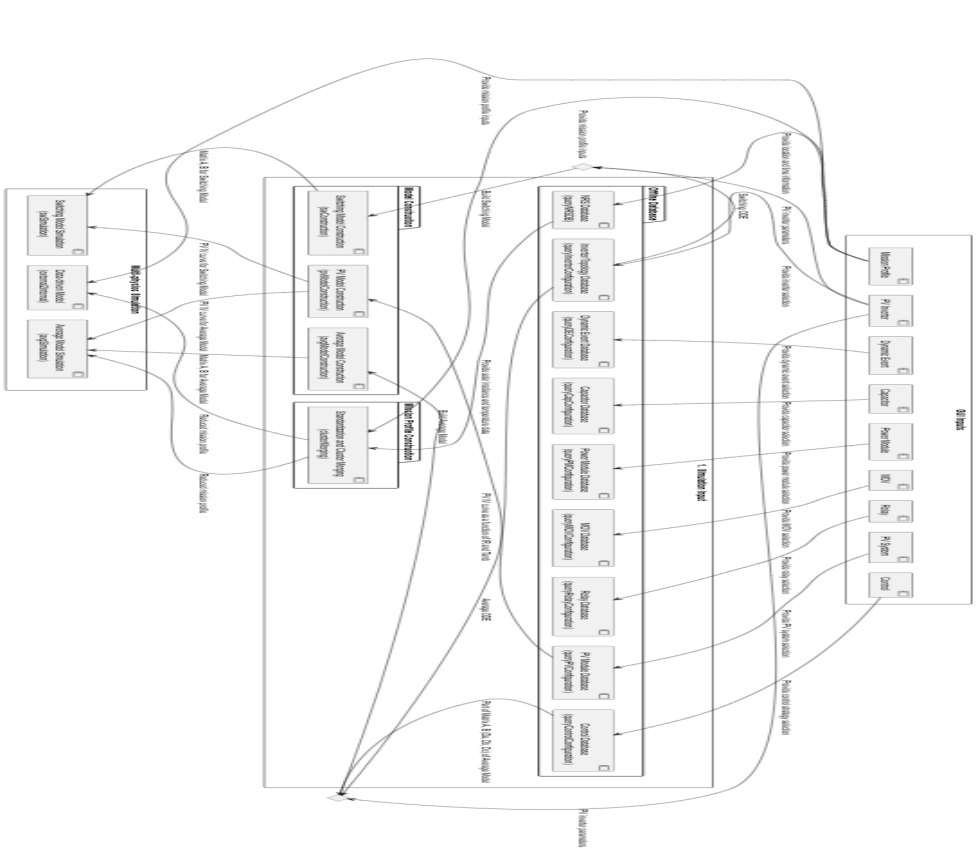
\includegraphics[width=\textwidth]{figure11..png}
    \caption{Simulation Preparation Dataflow}
\end{figure}

\subsection{Database query}
For each database established offline, necessary information can be queried via according to the primary key, which comes from the user inputs. The detail inputs and outputs for the query functions have been listed in the tables below.

\subsubsection{PV Module Database Query}
\begin{table}[h]
\centering
\caption{Function: queryPVConfiguration}
\begin{tabular}{|l|p{4cm}|p{2cm}|p{5cm}|p{2cm}|}
\hline
\multicolumn{5}{|l|}{\textbf{Input}} \\ \hline
\textbf{No.} & \textbf{Variable Name} & \textbf{Data Type} & \textbf{Description} & \textbf{From} \\ \hline
1 & PVModule.pvModulePartNumber & Enum & Part number of the PV module used in the system. & 1.2.1 \\ \hline
2 & ReducedMissionProfile.IR & float & I–V curves of the PV module under varying irradiance and temperature conditions. & 2.2 \\ \hline
3 & ReducedMissionProfile.Temp & float & Output voltage of the PV module. & 2.2 \\ \hline
4 & pvModuleDB & PVModuleDB & PV module I–V curve database. & 1.2.2 \\ \hline
5 & numberOfParallelStrings & Integer & Number of parallel-connected PV strings in the array. & 1.2.1 \\ \hline
6 & numberOfSeries & Integer & Number of series-connected modules in each string. & 1.2.1 \\ \hline
\multicolumn{5}{|l|}{\textbf{Output}} \\ \hline
\textbf{No.} & \textbf{Variable Name} & \textbf{Data Type} & \textbf{Description} & \textbf{To} \\ \hline
1 & pvIvCurve & float[] & I–V curves of the PV string considering the number of parallels and number of series under varying conditions. & 3.1.1 \\ \hline
2 & pvPVCurve & float[] & Output power vs. voltage of the PV module. & 3.1.1 \& 3.1.3 \\ \hline
\end{tabular}
\end{table}

\subsubsection{NRSDB Query}
\begin{table}[h]
\centering
\caption{NRSDB Query (Optional)}
\begin{tabular}{|l|l|l|p{5cm}|p{3cm}|}
\hline
\multicolumn{5}{|l|}{\textbf{Input}} \\ \hline
\textbf{No.} & \textbf{Variable Name} & \textbf{Data Type} & \textbf{Description} & \textbf{From} \\ \hline
1 & Latitude & Float & Latitude of the target location & 1.1.1 \\ \hline
2 & Longitude & Float & Longitude of the target location & 1.1.1 \\ \hline
3 & Year & integer & Calendar year of the record & 1.1.1 \\ \hline
4 & Interval & Integer & Time resolution of the record & 1.1.1 \\ \hline
\multicolumn{5}{|l|}{\textbf{Output}} \\ \hline
\textbf{No.} & \textbf{Variable Name} & \textbf{Data Type} & \textbf{Description} & \textbf{To} \\ \hline
5 & MissionProfile.IR & Float[] & Solar Irradiance (Environmental Condition) & 2.2 \& 3.3.1 \\ \hline
6 & MissionProfile.Tamb & Float[] & Ambient Temperature (Environmental Condition) & 2.2 \& 3.3.1 \\ \hline
7 & MissionProfile.RH & Float[] & Relative Humidity (Environmental Condition) & 2.2 \& 3.3.1 \\ \hline
\end{tabular}
\end{table}

\subsubsection{Control Database Query}
\begin{table}[h]
\centering
\caption{Function: queryControlConfiguration}
\begin{tabular}{|l|l|l|p{5cm}|p{3cm}|}
\hline
\multicolumn{5}{|l|}{\textbf{Input}} \\ \hline
\textbf{No.} & \textbf{Variable Name} & \textbf{Data Type} & \textbf{Description} & \textbf{From} \\ \hline
1 & Control.controlStrategy & Enum & Control parameter database for the PV inverter. & 1.4.2 \\ \hline
2 & controlDb & float[] & Control parameter database for the PV inverter. & 1.4.2 \\ \hline
\multicolumn{5}{|l|}{\textbf{Output}} \\ \hline
\textbf{No.} & \textbf{Variable Name} & \textbf{Data Type} & \textbf{Description} & \textbf{To} \\ \hline
1 & da & float[] & Duty ratio of phase A leg & 3.1.1 \\ \hline
2 & db & float[] & Duty ratio of phase B leg & 3.1.1 \\ \hline
3 & dc & float[] & Duty ratio of phase C leg & 3.1.1 \\ \hline
\end{tabular}
\end{table}

\subsubsection{Inverter/Topology Database Query}
\begin{table}[h]
\centering
\caption{Function: queryInverterConfiguration}
\begin{tabular}{|l|p{4cm}|p{2cm}|p{5cm}|p{2cm}|}
\hline
\multicolumn{5}{|l|}{\textbf{Input}} \\ \hline
\textbf{No.} & \textbf{Variable Name} & \textbf{Data type} & \textbf{Description} & \textbf{From} \\ \hline
1 & PVInverter.pvInverterPartNumber & PVModuleTopology & PV inverter Topology & 1.3.1 \\ \hline
2 & PVInverter.pvInverterModulationScheme & Modulation Scheme & PV inverter modulation scheme & 1.3.1 \\ \hline
3 & inverterDb & Float[] & PV inverter database & 1.3.2 \\ \hline
\multicolumn{5}{|l|}{\textbf{Output}} \\ \hline
\textbf{No.} & \textbf{Variable Name} & \textbf{Data type} & \textbf{Description} & \textbf{To} \\ \hline
1 & PVInverter.avgODE & Float[] & Average model ODE & 3.1.1 \\ \hline
2 & PVInverter.swODE & Float[] & Switching model ODE & 3.1.3 \\ \hline
\end{tabular}
\end{table}

\subsubsection{Inverter Modulation Database Query}
\begin{table}[h]
\centering
\caption{Function: queryInvertermodulationindexConfiguration}
\begin{tabular}{|l|p{4cm}|p{2cm}|p{5cm}|p{2cm}|}
\hline
\multicolumn{5}{|l|}{\textbf{Input}} \\ \hline
\textbf{No.} & \textbf{Variable Name} & \textbf{Data type} & \textbf{Description} & \textbf{From} \\ \hline
1 & PVInverter.pvInverterPartNumber & PVModuleTopology & PV inverter Topology & 1.3.1 \\ \hline
2 & PVInverter.pvInverterModulationScheme & Modulation Scheme & PV inverter modulation scheme & 1.3.1 \\ \hline
3 & Da & Float[] & Duty ratio of phase A leg & 2.1.3 \\ \hline
4 & Db & Float[] & Duty ratio of phase B leg & 2.1.3 \\ \hline
5 & Dc & Float[] & Duty ratio of phase C leg & 2.1.3 \\ \hline
6 & modulationschemeDb & Float[] & Modulation scheme database & 1.3.2 \\ \hline
\multicolumn{5}{|l|}{\textbf{Output}} \\ \hline
\textbf{No.} & \textbf{Variable Name} & \textbf{Data type} & \textbf{Description} & \textbf{To} \\ \hline
1 & Sa\_T & Float[] & Switching state function for the phase A leg vs. Time & 3.1.3 \\ \hline
2 & Sb\_T & Float[] & Switching state function for the phase B leg vs. Time & 3.1.3 \\ \hline
 & Sc\_T & Float[] & Switching state function for the phase C leg vs. Time & 3.1.3 \\ \hline
\end{tabular}
\end{table}

\subsubsection{Dynamic Event Database Query}
\begin{table}[h]
\centering
\caption{Function: queryDEConfiguration}
\begin{tabular}{|l|l|l|l|l|}
\hline
\multicolumn{5}{|l|}{\textbf{Input}} \\ \hline
\textbf{No.} & \textbf{Variable Name} & \textbf{Data type} & \textbf{Description} & \textbf{From} \\ \hline
1 & latitude & Float & Latitude of the target location & 1.5.1 \\ \hline
2 & longitude & Float & Longitude of the target location & 1.5.1 \\ \hline
3 & eventID & Integer & Dynamic event ID & 1.5.1 \\ \hline
4 & deDB & Float[] & Dynamic event database & 1.5.2 \\ \hline
\multicolumn{5}{|l|}{\textbf{Output}} \\ \hline
\textbf{No.} & \textbf{Variable Name} & \textbf{Data type} & \textbf{Description} & \textbf{To} \\ \hline
1 & eventType & Enum & Category or type of the dynamic event. & Xxx \\ \hline
2 & eventTime & Datatime & Timestamp indicating when the event occurs. & xxx \\ \hline
3 & eventDuration & float & Time span for which the event lasts. & xxx \\ \hline
\end{tabular}
\end{table}

\subsubsection{Capacitor Database Query}
\begin{table}[h]
\centering
\caption{Function: queryCapacitorConfiguration}
\begin{tabular}{|l|p{3cm}|l|p{6cm}|p{2cm}|}
\hline
\multicolumn{5}{|l|}{\textbf{Input}} \\ \hline
\textbf{No.} & \textbf{Variable Name} & \textbf{Data type} & \textbf{Description} & \textbf{From} \\ \hline
1 & Capacitor.capacitorPartNo & Enum & Capacitor Part Number & 1.6.2.1 \\ \hline
2 & Capacitor.capType & Enum & The type of capacitor & 1.6.2.1 \\ \hline
3 & capacitorDB & Float[] & Capacitor database & 1.6.2.2 \\ \hline
\multicolumn{5}{|l|}{\textbf{Output}} \\ \hline
\textbf{No.} & \textbf{Variable Name} & \textbf{Data type} & \textbf{Description} & \textbf{To} \\ \hline
1 & Capacitor.Capacitance\_T\_V & float & Capacitance value of the capacitor vs. Temperature and voltage & 3.2.1.1 \& 3.2.2.1 \\ \hline
2 & Capacitor.Esr\_T\_freq & float & Energy dissipated during diode reverse recovery vs. Temperature and frequency & 3.2.1.1 \\ \hline
3 & Capacitor.Rth\_ah & Float[] & Thermal resistance from ambient to hotspot & 3.2.2.1 \\ \hline
4 & Capacitor.Rth\_as & Float[] & Thermal resistance from ambient to surface & 3.2.2.1 \\ \hline
5 & Capacitor.Cap\_freq? & DC-link & DC-link capacitor frequency & 3.2.2.1 \\ \hline
6 & Capacitor.Cap\_reliability\_coef & Float[] & Capacitor reliability model coefficients & 4.2.2.1 \& 4.2.2.2 \\ \hline
7 & Capacitor.Capacitance\_T\_V & & Capacitance value of the capacitor vs. Temperature and voltage & \\ \hline
\end{tabular}
\end{table}

\subsubsection{Power Module Database Query}
\begin{table}[h]
\centering
\caption{Function: queryPMConfiguration}
\begin{tabular}{|l|p{3.5cm}|l|p{6cm}|p{1.5cm}|}
\hline
\multicolumn{5}{|l|}{\textbf{Input}} \\ \hline
\textbf{No.} & \textbf{Variable Name} & \textbf{Data type} & \textbf{Description} & \textbf{From} \\ \hline
1 & PowerModule.pmPartNo & Enum & Power module Part Number & 1.6.1.1 \\ \hline
2 & pmDb & Float[] & PV inverter database & 1.6.1.2 \\ \hline
\multicolumn{5}{|l|}{\textbf{Output}} \\ \hline
\textbf{No.} & \textbf{Variable Name} & \textbf{Data type} & \textbf{Description} & \textbf{To} \\ \hline
1 & PowerModule.rth & float & Thermal resistance of the power module. & 3.2.2.2 \\ \hline
2 & PowerModule.Von\_Ic\_Tj & Float[] & On-State Voltage vs. Collector current and temperature & 3.2.1.2 \\ \hline
3 & PowerModule.Eon\_Ic\_Vce & Float[] & The turn-on energy loss vs. inductor current and the blocking voltage & 3.2.1.2 \\ \hline
4 & PowerModule.Eoff\_Ic\_Vce & Float[] & The turn-off energy loss vs. Inductor current and the blocking voltage & 4.2.3.1.1 \\ \hline
5 & PowerModule. & Float[] & Reverse recovery energy loss vs. inductor current and the block voltage & 4.2.3.1.2 \& 4.2.3.2 \\ \hline
\end{tabular}
\end{table}

\subsubsection{PCB Database Query}
\begin{table}[h]
\centering
\caption{Function: queryPCBConfiguration}
\begin{tabular}{|l|p{3cm}|l|p{6cm}|l|}
\hline
\multicolumn{5}{|l|}{\textbf{Input}} \\ \hline
\textbf{No.} & \textbf{Variable Name} & \textbf{Data type} & \textbf{Description} & \textbf{From} \\ \hline
1 & PCB.footprint & Enum & The footprint soldered on the PCB & 1.6.3.1 \\ \hline
2 & PCB.solderJoint material & Enum & The material of the solder joint & 1.6.3.1 \\ \hline
3 & PCB.Thickness & Float & The thickness of PCB & 1.6.3.1 \\ \hline
4 & PCB.Dimension & & Physical dimensions of the PCB & 1.6.3.1 \\ \hline
5 & PCBDB & Float[] & PCB Database & 1.6.3.2 \\ \hline
\multicolumn{5}{|l|}{\textbf{Output}} \\ \hline
\textbf{No.} & \textbf{Variable Name} & \textbf{Data type} & \textbf{Description} & \textbf{To} \\ \hline
1 & PCB\_reliability\_coef & float[] & Physical dimensions of the PCB. & 4.2.4 \\ \hline
\end{tabular}
\end{table}

\subsubsection{Cooling Fan Database Query}
\begin{table}[h]
\centering
\caption{Function: queryCoolingFanConfiguration}
\begin{tabular}{|l|p{4cm}|l|p{5cm}|l|}
\hline
\multicolumn{5}{|l|}{\textbf{Input}} \\ \hline
\textbf{No.} & \textbf{Variable Name} & \textbf{Data type} & \textbf{Description} & \textbf{From} \\ \hline
1 & CoolingFan.coolingFanPartNumber & Enum & Cooling Fan Part Number & 1.6.4.1 \\ \hline
2 & CoolingFanDb & Float[] & Cooling Fan database & 1.6.4.2 \\ \hline
\multicolumn{5}{|l|}{\textbf{Output}} \\ \hline
\textbf{No.} & \textbf{Variable Name} & \textbf{Data type} & \textbf{Description} & \textbf{To} \\ \hline
1 & CoolingFan.CoolingFan\_reliability\_coef\_mechanical & float[] & Cooling fan reliability model coefficient considering mechanical failure & 4.2.1.1 \\ \hline
2 & CoolingFan.CoolingFan\_reliability\_coef\_electrical & float[] & Cooling fan reliability model coefficient considering electrical failure & 4.2.1.2 \\ \hline
\end{tabular}
\end{table}

\subsubsection{MOV Database Query}
\begin{table}[h]
\centering
\caption{Function: queryMOVConfiguration}
\begin{tabular}{|l|l|l|l|l|}
\hline
\multicolumn{5}{|l|}{\textbf{Input}} \\ \hline
\textbf{No.} & \textbf{Variable Name} & \textbf{Data type} & \textbf{Description} & \textbf{From} \\ \hline
1 & movPartNo & Enum & MOV Part Number & 1.6.5.1 \\ \hline
2 & movDb & Float[] & MOV database & 1.6.5.2 \\ \hline
\multicolumn{5}{|l|}{\textbf{Output}} \\ \hline
\textbf{No.} & \textbf{Variable Name} & \textbf{Data type} & \textbf{Description} & \textbf{To} \\ \hline
1 & movIVCurve & float[] & Current–voltage characteristic curve of the device. & xxx \\ \hline
2 & movPulseRatingCurve & float[] & Lifetime curve of the device under electrical cycling stress. & xxx \\ \hline
\end{tabular}
\end{table}

\subsubsection{Relay Database Query}
\begin{table}[h]
\centering
\caption{Function: queryRelayConfiguration}
\begin{tabular}{|l|l|l|l|l|}
\hline
\multicolumn{5}{|l|}{\textbf{Input}} \\ \hline
\textbf{No.} & \textbf{Variable Name} & \textbf{Data type} & \textbf{Description} & \textbf{From} \\ \hline
1 & relayPartNo & Enum & Relay Part Number & 1.6.6.1 \\ \hline
2 & relayDb & Float[] & Relay database & 1.6.6.2 \\ \hline
\multicolumn{5}{|l|}{\textbf{Output}} \\ \hline
\textbf{No.} & \textbf{Variable Name} & \textbf{Data type} & \textbf{Description} & \textbf{To} \\ \hline
1 & relayIVCurve & float[] & Current–voltage characteristic curve of the device. & xxx \\ \hline
2 & relayPulseRatingCurve & float[] & Lifetime curve of the device under electrical cycling stress. & xxx \\ \hline
\end{tabular}
\end{table}

\subsection{Cluster Merging}
\begin{table}[h]
\centering
\caption{Function: clusterMerging}
\begin{tabular}{|l|l|p{6cm}|l|l|}
\hline
\multicolumn{5}{|l|}{\textbf{Input}} \\ \hline
\textbf{No.} & \textbf{Variable Name} & \textbf{Description} & \textbf{Data type} & \textbf{From} \\ \hline
1 & MissionProfile.missionProfile & Full mission profile & missionProfile & 1.1.1 \& 1.1.2 \\ \hline
2 & mfTolerance & Pre-defined Similarity Threshold & Float & 1.7 \\ \hline
\multicolumn{5}{|l|}{\textbf{Output}} \\ \hline
\textbf{No.} & \textbf{Variable Name} & \textbf{Description} & \textbf{Data type} & \textbf{To} \\ \hline
1 & ReducedMissionProfile & Reduced Mission Profile & missionProfile & 2.1.1, 3.3.1, 4.2.1.1, 4.2.1.2 \\ \hline
2 & hashTable & Recovery Map & float[] & 5. \\ \hline
\end{tabular}
\end{table}

\section{Multi-physics Simulator}
\begin{figure}[h]
    \centering
    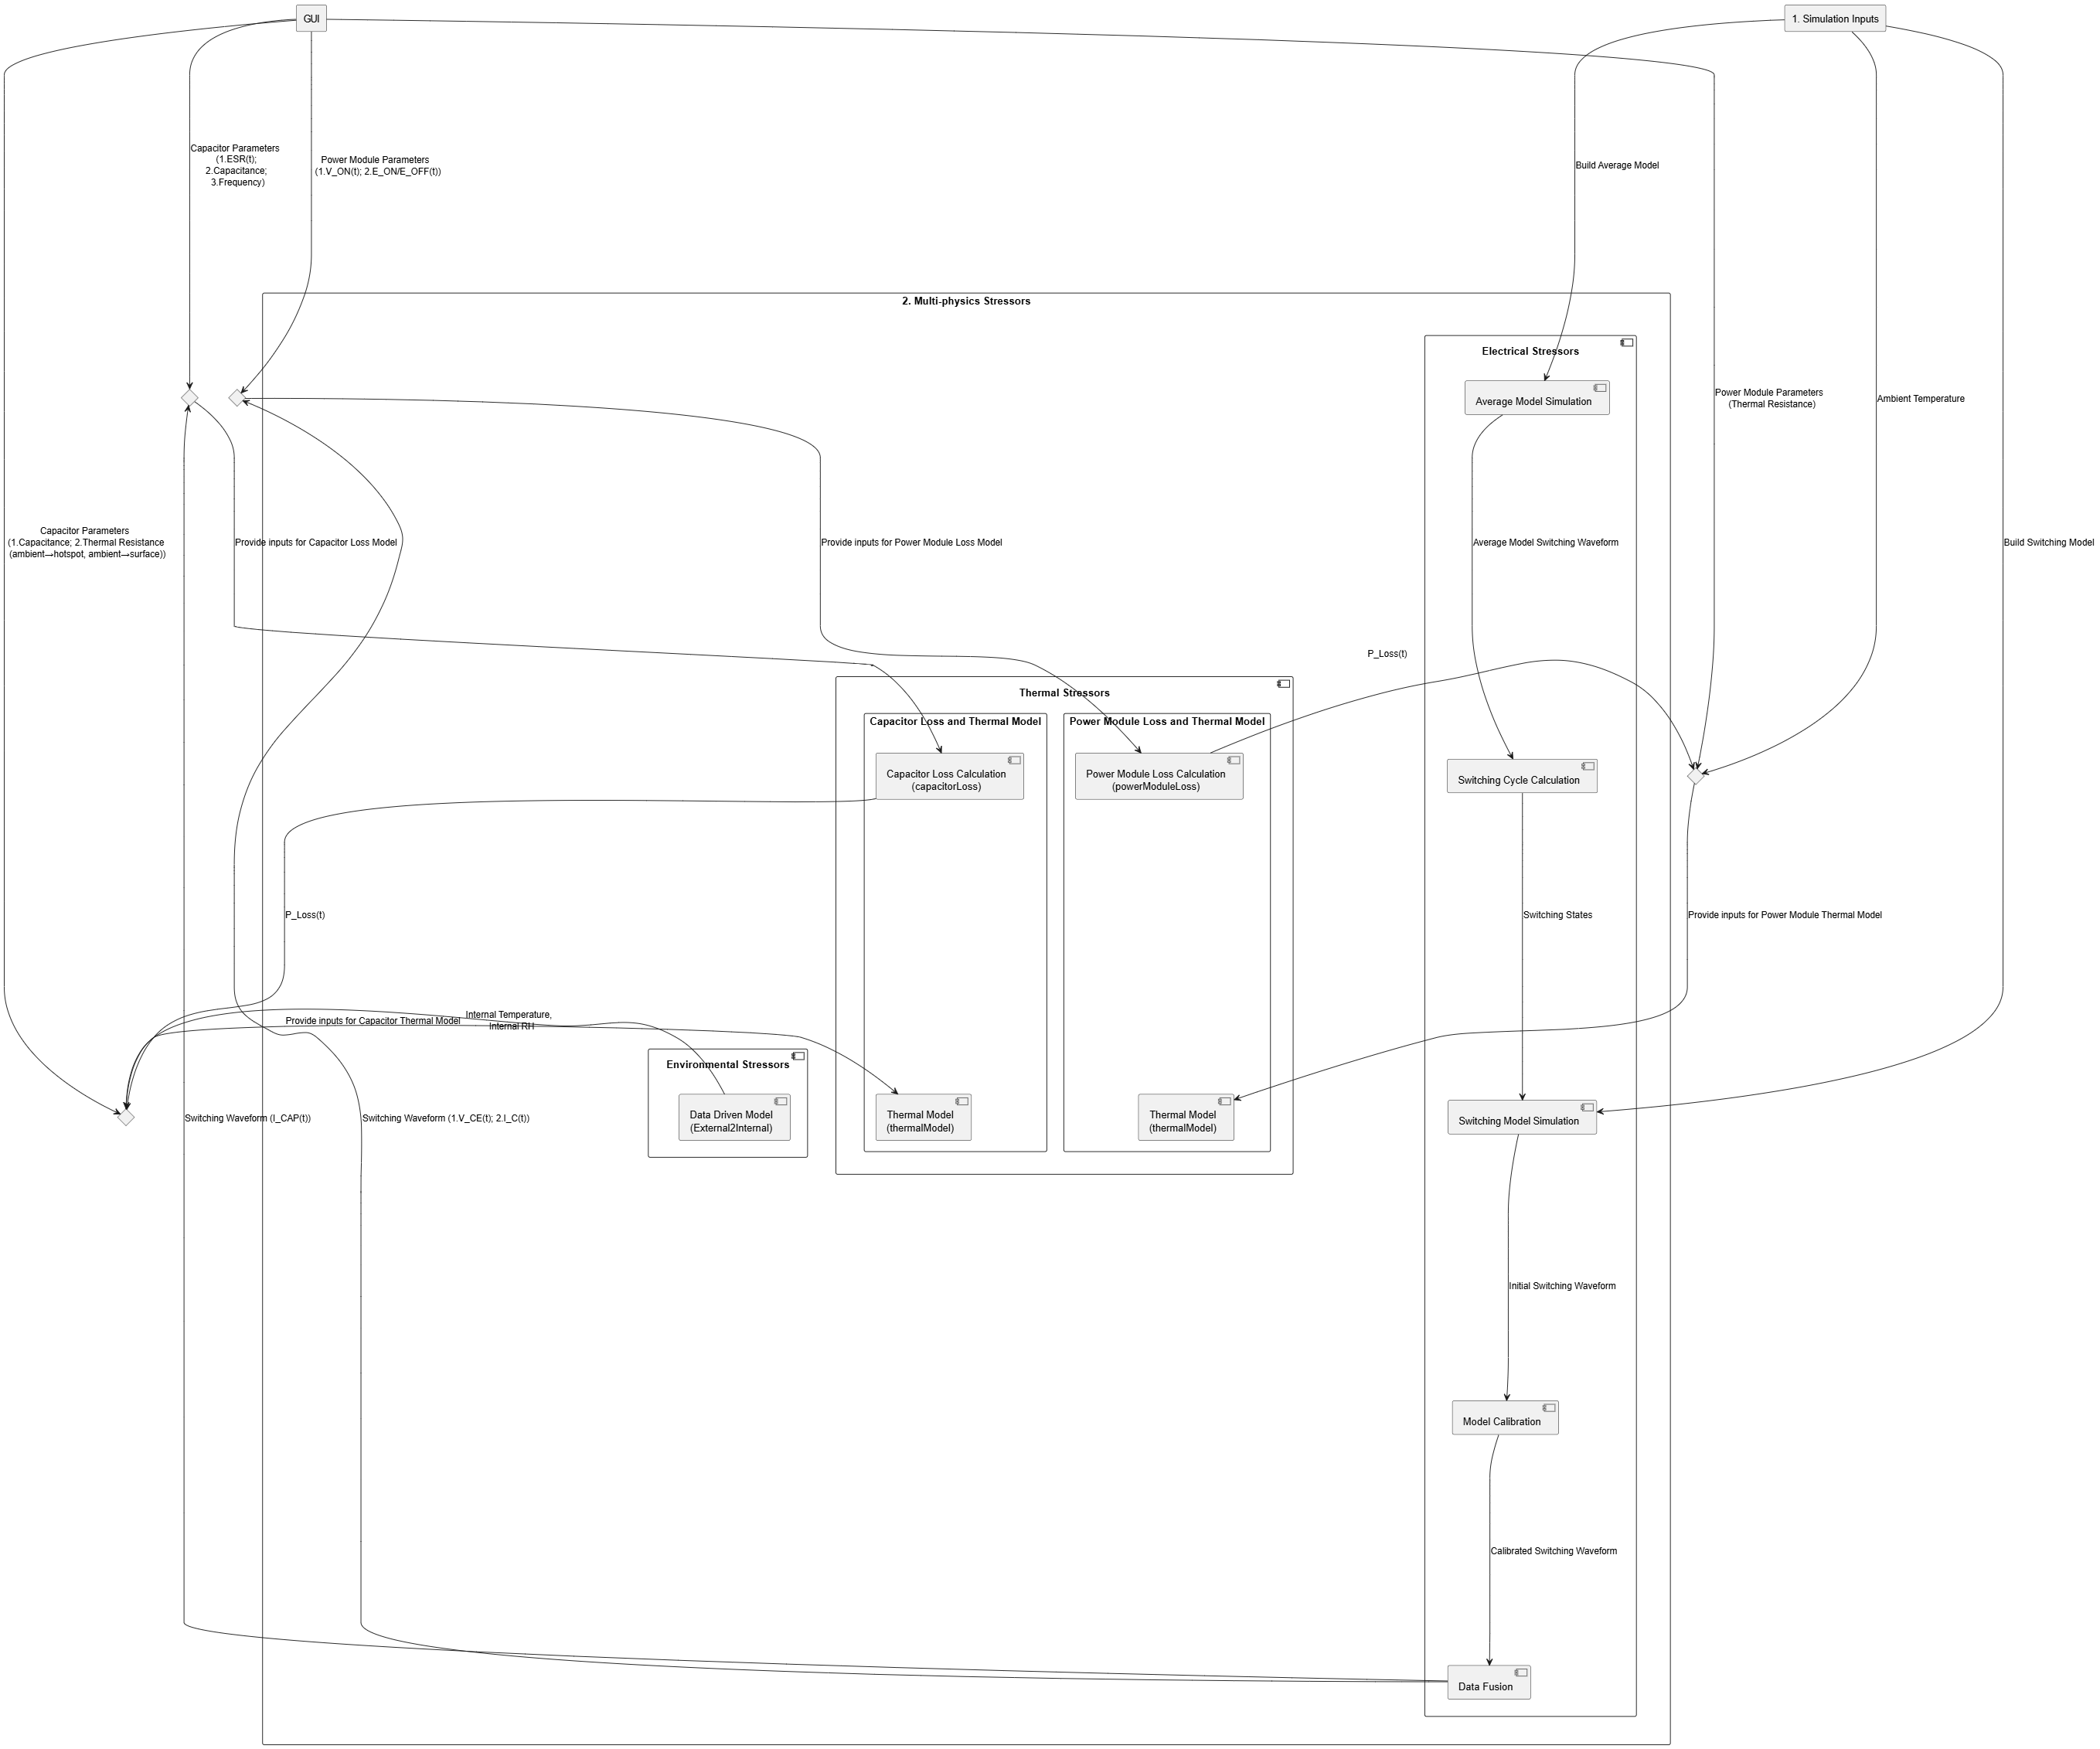
\includegraphics[width=\textwidth]{figure12.png}
    \caption{Multi-physics Simulator Dataflow}
\end{figure}

\subsection{Electrical Simulation}
\subsubsection{Average Model Simulation}
\begin{table}[h]
\centering
\caption{Function: avgModelSimulation}
\begin{tabular}{|l|p{3.5cm}|p{5cm}|l|p{2cm}|}
\hline
\multicolumn{5}{|l|}{\textbf{Input}} \\ \hline
\textbf{No.} & \textbf{Variable Name} & \textbf{Description} & \textbf{Data type} & \textbf{From} \\ \hline
1 & Simulation\_time & Simulation Time & Float & 1.7 \\ \hline
2 & PVInverter.f\_inv\_sw & Switching frequency of the inverter & Float & 2.1.4 \\ \hline
3 & phaseShift & Phase Shift of the waveform & Float & 1.7 \\ \hline
4 & reducedMissionProfile.Vdc & DC voltage from the reduced mission profile & Float[] & 2.2 \\ \hline
5 & reducedMissionProfile.Vac & AC voltage from the reduced mission profile & Float[] & 2.2 \\ \hline
6 & gridVoltage & Nominal voltage level of the grid connection & Float[] & 1.2.1 \\ \hline
7 & gridFrequency & Operating frequency of the grid & Float[] & 1.2.1 \\ \hline
8 & gridPhase & Phase type of the grid connection & Enum & 1.2.1 \\ \hline
9 & V\_PV & PV module output voltage & Float[] & 2.1.1 \\ \hline
10 & da & N/A & Float[] & 2.1.5 \\ \hline
11 & db & N/A & Float[] & 2.1.5 \\ \hline
12 & dc & N/A & Float[] & 2.1.5 \\ \hline
13 & Timestep & s & Float & 1.7 \\ \hline
\multicolumn{5}{|l|}{\textbf{Output}} \\ \hline
\textbf{No.} & \textbf{Variable Name} & \textbf{Description} & \textbf{Data type} & \textbf{To} \\ \hline
1 & I1\_avg & Average Converter side AC inductor current & Float[] & 3.1.3 \\ \hline
2 & I2\_avg & Average Grid side AC inductor current & float[] & 3.1.3 \\ \hline
3 & Vc\_avg & Average AC filter capacitor voltage & Float[] & 3.1.3 \\ \hline
4 & I\_Lboost\_avg & Average DC boost inductor current & Float[] & 3.1.3 \\ \hline
5 & V\_CDC1\_avg & Average Upper split DC-link capacitor voltage & Float[] & 3.1.3 \\ \hline
6 & V\_CDC2\_avg & Average Lower split DC-link capacitor voltage & Float[] & 3.1.3 \\ \hline
\end{tabular}
\end{table}

\subsubsection{A2S Simulation}
\begin{table}[h]
\centering
\caption{Function: a2sSimulation}
\begin{tabular}{|l|l|p{6cm}|l|l|}
\hline
\multicolumn{5}{|l|}{\textbf{Input}} \\ \hline
... & ... & ... & ... & ... \\ \hline
\multicolumn{5}{|p{15cm}|}{*(The variables listed mirror the average model simulation above with states from 3.1.1 and switching state functions from 2.1.5)*} \\ \hline
\multicolumn{5}{|l|}{\textbf{Output}} \\ \hline
\textbf{No.} & \textbf{Variable Name} & \textbf{Description} & \textbf{Data type} & \textbf{To} \\ \hline
1 & Icap & Instantaneous current flowing through the DC-link capacitor & Float[] & 3.2.1.1 \\ \hline
2 & V\_CE & Collector–Emitter Voltage vs. Time & Float[] & 3.2.1.2 \\ \hline
3 & I\_C & Collector Current vs. Time & Float[] & 3.2.1.2 \\ \hline
4 & ac\_power & AC Power & Float[] & 3.2.1.2 \\ \hline
\end{tabular}
\end{table}

\subsection{Thermal Simulation}
\subsubsection{Loss Model}
\paragraph{Capacitor Loss Model}
\begin{table}[h]
\centering
\caption{Function: capLossCalculation}
\begin{tabular}{|l|l|p{6cm}|l|l|}
\hline
\multicolumn{5}{|l|}{\textbf{Input}} \\ \hline
\textbf{No.} & \textbf{Variable Name} & \textbf{Description} & \textbf{Data type} & \textbf{From} \\ \hline
1 & Icap & Instantaneous current flowing through the DC-link capacitor & Float & 3.1 \\ \hline
2 & capacitor.ESR & Capacitor ESR & Float[] & 2.1.7 \\ \hline
3 & capacitor.capacitance & DC-link capacitor capacitance & Float[] & 2.1.7 \\ \hline
4 & capacitor.frequency & DC-link capacitor frequency & Float[] & 2.1.7 \\ \hline
\multicolumn{5}{|l|}{\textbf{Output}} \\ \hline
\textbf{No.} & \textbf{Variable Name} & \textbf{Description} & \textbf{Data type} & \textbf{To} \\ \hline
1 & Loss\_cap & Capacitor loss vs. Function of Temperature & Float[] & 3.2 \\ \hline
\end{tabular}
\end{table}

\paragraph{Power Module Loss Model}
\begin{table}[h]
\centering
\caption{Function: pmLossCalculation}
\begin{tabular}{|l|l|p{6cm}|l|l|}
\hline
\multicolumn{5}{|l|}{\textbf{Input}} \\ \hline
\textbf{No.} & \textbf{Variable Name} & \textbf{Description} & \textbf{Data type} & \textbf{From} \\ \hline
1 & V\_CE & Collector Current vs. Time & Float[] & 3.1 \\ \hline
2 & I\_C & Collector–Emitter Voltage vs. Time & Float[] & 3.1 \\ \hline
3 & V\_on & On-state voltage drop vs. Time & Float[] & 2.1.8 \\ \hline
4 & E\_on/off & Turn-on/off energy loss vs. Time & Float[] & 2.1.8 \\ \hline
\multicolumn{5}{|l|}{\textbf{Output}} \\ \hline
\textbf{No.} & \textbf{Variable Name} & \textbf{Description} & \textbf{Data type} & \textbf{To} \\ \hline
1 & Loss\_pm & Power Module loss vs. Function of Temperature & Float[] & 3.2.2.2 \\ \hline
\end{tabular}
\end{table}

\subsubsection{Thermal Model}
\paragraph{Capacitor Thermal Model}
\begin{table}[h]
\centering
\caption{Function: capThermalCalculation}
\begin{tabular}{|l|l|p{6cm}|l|l|}
\hline
\multicolumn{5}{|l|}{\textbf{Input}} \\ \hline
\textbf{No.} & \textbf{Variable Name} & \textbf{Description} & \textbf{Data type} & \textbf{From} \\ \hline
1 & Loss\_cap & Capacitor loss vs. Function of Temperature & Float[] & 3.1 \\ \hline
2 & capacitor.Rth & Capacitor Rth & Float[] & 2.1.7 \\ \hline
3 & capacitor.capacitance & DC-link capacitor capacitance & Float[] & 2.1.7 \\ \hline
4 & Internal\_temp & Internal temperature within PV inverter enclosure & Float[] & 3.3.1 \\ \hline
5 & Internal\_rh & Internal relative humidity within PV inverter enclosure & Float[] & 3.3.1 \\ \hline
\multicolumn{5}{|l|}{\textbf{Output}} \\ \hline
\textbf{No.} & \textbf{Variable Name} & \textbf{Description} & \textbf{Data type} & \textbf{To} \\ \hline
1 & T\_hotspot\_cap & Capacitor hotspot Temperature & Float & 4.2.2.1 \& 4.2.2.2 \\ \hline
2 & T\_surface\_cap & Capacitor surface temperature & Float & 4.2.2.1 \& 4.2.2.2 \\ \hline
\end{tabular}
\end{table}

\paragraph{Power Module Thermal Model}
\begin{table}[h]
\centering
\caption{Function: pmThermalCalculation}
\begin{tabular}{|l|l|p{6cm}|l|l|}
\hline
\multicolumn{5}{|l|}{\textbf{Input}} \\ \hline
\textbf{No.} & \textbf{Variable Name} & \textbf{Description} & \textbf{Data type} & \textbf{From} \\ \hline
1 & Loss\_pm & Power module loss vs. Function of temperature & Float[] & 3.2.1.2 \\ \hline
2 & reducedMissionProfile.Tamb & Reduced ambient temperature & Float & 2.2 \\ \hline
3 & powerModule.Rth & Thermal resistance vs. Time & Float[] & 2.1.8 \\ \hline
\multicolumn{5}{|l|}{\textbf{Output}} \\ \hline
\textbf{No.} & \textbf{Variable Name} & \textbf{Description} & \textbf{Data type} & \textbf{To} \\ \hline
1 & Tj & Power module junction temperature & Float & 4.2.3.1 \& 4.2.3.2 \\ \hline
\end{tabular}
\end{table}

\subsection{Environmental Simulation}
\subsubsection{External2Internal Model}
\begin{table}[h]
\centering
\caption{Function: external2internal}
\begin{tabular}{|l|l|p{5cm}|l|l|}
\hline
\multicolumn{5}{|l|}{\textbf{Input}} \\ \hline
\textbf{No.} & \textbf{Variable Name} & \textbf{Description} & \textbf{Data type} & \textbf{From} \\ \hline
1 & MissionProfile.temp & Ambient temperature & Float[] & 1.1.1.1 \& 2.1.2 \\ \hline
2 & MissionProfile.rh & Relative humidity & Float[] & 1.1.1.1 \& 2.1.2 \\ \hline
3 & MissionProfile.ac\_power & AC power & Float[] & 3.1.3 \\ \hline
\multicolumn{5}{|l|}{\textbf{Output}} \\ \hline
\textbf{No.} & \textbf{Variable Name} & \textbf{Description} & \textbf{Data type} & \textbf{To} \\ \hline
1 & Internal\_temp & Internal temperature within PV inverter & Float[] & 3.1.3 \\ \hline
2 & Internal\_rh & Internal RH within PV inverter & Float[] & 3.1.3 \\ \hline
\end{tabular}
\end{table}

\section{Reliability Assessment}
\subsection{Rainflow Counting Algorithm}
\begin{table}[h]
\centering
\caption{Function: rainflowCounting}
\begin{tabular}{|l|l|p{6cm}|l|l|}
\hline
\multicolumn{5}{|l|}{\textbf{Input}} \\ \hline
\textbf{No.} & \textbf{Variable Name} & \textbf{Description} & \textbf{Data type} & \textbf{From} \\ \hline
1 & hotspotTemp & Hotspot Temperature / Junction Temperature & Float[] & 3.2.2.2 \& 3.3.1 \\ \hline
\multicolumn{5}{|l|}{\textbf{Output}} \\ \hline
\textbf{No.} & \textbf{Variable Name} & \textbf{Description} & \textbf{Data type} & \textbf{To} \\ \hline
1 & deltaTRange & Temperature swing & Float[] & 4.2.3.1.1, 4.2.3.2, 4.2.4 \\ \hline
2 & deltaTCycle & Full/Half cycle & Float[] & 4.2.3.1.1, 4.2.3.2, 4.2.4 \\ \hline
3 & Tjmax & Maximum junction temperature & Float[] & 4.2.3.1.1, 4.2.3.2, 4.2.4 \\ \hline
\end{tabular}
\end{table}

\subsection{Reliability Assessment for each component}
\subsubsection{Cooling Fan}
\paragraph{Cooling fan mechanical model}
\begin{table}[h]
\centering
\caption{Function: coolingFanLifetimeEstimation\_mechanical}
\begin{tabular}{|l|p{4cm}|p{4cm}|l|l|}
\hline
\multicolumn{5}{|l|}{\textbf{Input}} \\ \hline
\textbf{No.} & \textbf{Variable Name} & \textbf{Description} & \textbf{Data type} & \textbf{From} \\ \hline
1 & reduceMissionProfile.temp / internal\_temp & Ambient temperature / internal temperature & Float[] & 2.2 or 3.3.1 \\ \hline
\multicolumn{5}{|l|}{\textbf{Output}} \\ \hline
\textbf{No.} & \textbf{Variable Name} & \textbf{Description} & \textbf{Data type} & \textbf{To} \\ \hline
1 & coolingCurrLifetime\_mechanical & Cooling Fan current lifetime & Float[] & 5. \\ \hline
2 & coolingFanAccuDamage\_mechanical & Cooling Fan Cumulative Damage & Float[] & 5. \\ \hline
\end{tabular}
\end{table}

\paragraph{Cooling fan electrical model}
\begin{table}[h]
\centering
\caption{Function: coolingFanLifetimeEstimation\_electrical}
\begin{tabular}{|l|p{4cm}|p{4cm}|l|l|}
\hline
\multicolumn{5}{|l|}{\textbf{Input}} \\ \hline
\textbf{No.} & \textbf{Variable Name} & \textbf{Description} & \textbf{Data type} & \textbf{From} \\ \hline
1 & reduceMissionProfile.temp / internal\_temp & Ambient temperature / internal temperature & Float[] & 2.2 / 3.3.1 \\ \hline
2 & reduceMissionProfile.temp / internal\_rh & External RH / internal RH & Float[] & 2.2 / 3.3.1 \\ \hline
\multicolumn{5}{|l|}{\textbf{Output}} \\ \hline
\textbf{No.} & \textbf{Variable Name} & \textbf{Description} & \textbf{Data type} & \textbf{To} \\ \hline
1 & coolingCurrLifetime & Cooling Fan current lifetime & Float[] & 5. \\ \hline
2 & coolingFanAccuDamage & Cooling Fan Cumulative Damage & Float[] & 5. \\ \hline
\end{tabular}
\end{table}

\subsubsection{Capacitor}
\paragraph{Capacitor Lifetime Model}
\begin{table}[h]
\centering
\caption{Function: capacitorLifetimeEstimation}
\begin{tabular}{|l|l|l|l|l|}
\hline
\multicolumn{5}{|l|}{\textbf{Input}} \\ \hline
\textbf{No.} & \textbf{Variable Name} & \textbf{Description} & \textbf{Data type} & \textbf{From} \\ \hline
1 & reducedMissionProfile\_dc\_voltage & Operating Voltage & Float[] & 2.2 / 3.3.1 \\ \hline
2 & hotspotTemp & Operating Temperature & Float[] & 3.2.1.1 \\ \hline
3 & Internal\_rh & Operating RH & Float[] & 3.3.1 \\ \hline
4 & capcitorType & Capacitor Type & eunm & 2.1.7 \\ \hline
5 & capacitorCoeff & Reliability Coefficients & Float & 2.1.7 \\ \hline
\multicolumn{5}{|l|}{\textbf{Output}} \\ \hline
\textbf{No.} & \textbf{Variable Name} & \textbf{Description} & \textbf{Data type} & \textbf{To} \\ \hline
1 & capCurrLifetime & Capacitor current lifetime & Float[] & 5. \\ \hline
2 & capAccuDamage & Capacitor Cumulative Damage & Float & 5. \\ \hline
\end{tabular}
\end{table}

\paragraph{Capacitor Degradation Model}
\begin{table}[h]
\centering
\caption{Function: capacitorDegradation}
\begin{tabular}{|l|l|l|l|l|}
\hline
\multicolumn{5}{|l|}{\textbf{Input}} \\ \hline
\textbf{No.} & \textbf{Variable Name} & \textbf{Description} & \textbf{Data type} & \textbf{From} \\ \hline
1 & reducedMissionProfile\_ac\_voltage & Operating Voltage & Float[] & 2.2 / 3.3.1 \\ \hline
2 & hotspotTemp & Operating Temperature & Float[] & 3.2.1.1 \\ \hline
3 & Internal\_rh & Operating RH & Float[] & 3.3.1 \\ \hline
4 & capcitorType & Capacitor Type & eunm & 2.1.7 \\ \hline
5 & capacitorCoeff & Coefficient & Float & 2.1.7 \\ \hline
6 & Capacitor.ESR & Capacitor Equivalent Series Resistance & Float[] & 1.6.2 \\ \hline
\multicolumn{5}{|l|}{\textbf{Output}} \\ \hline
\textbf{No.} & \textbf{Variable Name} & \textbf{Description} & \textbf{Data type} & \textbf{To} \\ \hline
1 & capCurrLifetime & Capacitor current lifetime & Float[] & 5. \\ \hline
2 & capAccuDamage & Capacitor Cumulative Damage & Float[] & 5. \\ \hline
\end{tabular}
\end{table}

\subsubsection{Power Module}
\paragraph{Power Module Thermal Lifetime Model}
\begin{table}[h]
\centering
\caption{Function: PMLifetimeEstimation\_thermal}
\begin{tabular}{|l|l|l|l|l|}
\hline
\multicolumn{5}{|l|}{\textbf{Input}} \\ \hline
\textbf{No.} & \textbf{Variable Name} & \textbf{Description} & \textbf{Data type} & \textbf{From} \\ \hline
1 & deltaTRange & Temperature swing & Float[] & 4.1 \\ \hline
2 & deltaTCycle & Full/Half cycle & Float[] & 4.1 \\ \hline
3 & Tjmax & Maximum junction temperature & Float[] & 4.1 \\ \hline
4 & PM\_coef\_thermal & Reliability model coefficients & Float[] & 2.1.8 \\ \hline
\multicolumn{5}{|l|}{\textbf{Output}} \\ \hline
\textbf{No.} & \textbf{Variable Name} & \textbf{Description} & \textbf{Data type} & \textbf{To} \\ \hline
1 & PMCurrLifetime\_thermal & Power module current lifetime & Float[] & 5. \\ \hline
2 & PMAccuDamageRate\_thermal & Power module cumulative damage Rate & Float & 5. \\ \hline
\end{tabular}
\end{table}

\paragraph{Power Module RH Lifetime Model}
\begin{table}[h]
\centering
\caption{Function: PMLifetimeEstimation\_rh}
\begin{tabular}{|l|l|l|l|l|}
\hline
\multicolumn{5}{|l|}{\textbf{Input}} \\ \hline
\textbf{No.} & \textbf{Variable Name} & \textbf{Description} & \textbf{Data type} & \textbf{From} \\ \hline
1 & junction\_temp & Junction temperature for one month & Float[] & 3.2.2.2 \\ \hline
2 & Internal\_rh & Internal temperature for one month & Float[] & 3.3.1 \\ \hline
\multicolumn{5}{|l|}{\textbf{Output}} \\ \hline
\textbf{No.} & \textbf{Variable Name} & \textbf{Description} & \textbf{Data type} & \textbf{To} \\ \hline
1 & PMCurrLifetime\_rh & Power module current lifetime & Float[] & 5. \\ \hline
2 & PMAccuDamageRate\_rh & Power module cumulative damage Rate & Float & 5. \\ \hline
\end{tabular}
\end{table}

\subsubsection{PCB Lifetime Model}
\begin{table}[h]
\centering
\caption{Function: PCBLifetimeEstimation}
\begin{tabular}{|l|l|l|l|l|}
\hline
\multicolumn{5}{|l|}{\textbf{Input}} \\ \hline
\textbf{No.} & \textbf{Variable Name} & \textbf{Description} & \textbf{Data type} & \textbf{From} \\ \hline
1 & deltaTRange & Temperature swing & Float[] & 4.1 \\ \hline
2 & deltaTCycle & Full/Half cycle & Float[] & 4.1 \\ \hline
3 & dimension\_PCB & PCB dimension information & Float[] & 1.6.3 \\ \hline
4 & Solder\_joint\_PCB & PCB solder joint type & Enum & 1.6.3 \\ \hline
\multicolumn{5}{|l|}{\textbf{Output}} \\ \hline
\textbf{No.} & \textbf{Variable Name} & \textbf{Description} & \textbf{Data type} & \textbf{To} \\ \hline
1 & PCBCurrLifetime & PCB current lifetime & Float[] & 5. \\ \hline
2 & AccuDamageRate\_PCB & PCB cumulative damage Rate & Float & 5. \\ \hline
\end{tabular}
\end{table}

\subsubsection{MOV Lifetime Model}
(will be updated later)

\subsubsection{Relay Lifetime Model}
(will be updated later)

\section{LCOE, EOL and history stressors}
\begin{enumerate}
    \item accumulated damage
    \item Lifetime of inverter
    \item Which failure mechanism
    \item failed component
\end{enumerate}

\subsection{Component Lifetime Estimation}
\begin{table}[h]
\centering
\caption{Function: ComponentLifetimeEstimation}
\begin{tabular}{|l|p{4cm}|p{5cm}|l|l|}
\hline
\multicolumn{5}{|l|}{\textbf{Input}} \\ \hline
\textbf{No.} & \textbf{Variable Name} & \textbf{Description} & \textbf{Data type} & \textbf{From} \\ \hline
1 & coolingCurrLifetime\_mechanical & Current cooling fan lifetime considering mechanical failure mechanism & Float[] & 4.2.1.1 \\ \hline
2 & coolingCurrLifetime\_electrical & Current cooling fan lifetime considering electrical failure mechanism & Float[] & 4.2.1.2 \\ \hline
3 & capCurrLifetime & Capacitor current lifetime & Float[] & 4.2.2.1 \\ \hline
4 & PMCurrLifetime\_thermal & Number of cycles for power module within one month & Float[] & 4.2.3.1.1 \\ \hline
5 & PMCurrLifetime\_rh & Power module current lifetime considering the RH model & Float[] & 4.2.3.1.2 \\ \hline
6 & PCBCurrLifetime & PCB current lifetime & Float[] & 4.2.4 \\ \hline
7 & MOVCurrLifetime & xxx & xxx & 4.2.5 \\ \hline
8 & RelayCurrLifetime & xxx & xxx & 4.2.6 \\ \hline
\multicolumn{5}{|l|}{\textbf{Output}} \\ \hline
\textbf{No.} & \textbf{Variable Name} & \textbf{Description} & \textbf{Data type} & \textbf{To} \\ \hline
1 & ComponentStatus & Indicate if exists component failed & Float[] & Xxx \\ \hline
\end{tabular}
\end{table}

\clearpage
\section{Software Function Implementations}
\label{sec:function-implementations}
This section connects the workflow described in Sections 1--5 to the functions
implemented in the TRACE-PV source tree.  The listings intentionally show the
calculation and data-handling cores; CUDA allocation, diagnostic output, and
repetitive error handling are omitted where they do not change the algorithm.

\subsection{Mission-profile ingestion and case construction}
\label{sec:implementation-mission}
The function \texttt{load\_mission\_profile\_csv()} in
\texttt{src/simulation\_preparation/mission\_profile\_loader.cpp} converts each
CSV record into a \texttt{SimulationCase}.  The supported full record is
\texttt{time, ambient\_temperature, rh, solar\_irradiance, ac\_voltage,
ac\_power}.  AC power is therefore taken directly from the mission profile when
the sixth field is present; \texttt{has\_ac\_power} prevents an absent value from
being mistaken for a measured zero.  Records without positive irradiance or AC
voltage are excluded from the operating simulation.

\begin{lstlisting}[language=C++,caption={Mission-profile row parsing and operating-point filtering}]
SimulationCase sc;
sc.time = tokens[0];
sc.ambient_temperature = std::stod(tokens[1]);
sc.rh = std::stod(tokens[2]);
sc.solar_irradiance = std::stod(tokens[3]);
sc.ac_voltage = std::stod(tokens[4]);
if (tokens.size() >= 6 && !tokens[5].empty()) {
    sc.ac_power = std::stod(tokens[5]);
    sc.has_ac_power = true;
}
if (sc.solar_irradiance <= 0.0 || sc.ac_voltage <= 0.0) {
    continue;
}
cases.push_back(sc);
\end{lstlisting}

\subsection{Component-database query}
\label{sec:implementation-database}
\texttt{ComponentDatabase::load\_capacitor()} implements the capacitor query
defined in Section 2.1.6.  A parameterized SQLite statement selects the
reliability, electrical, and thermal coefficients by part number.  The function
maps the stored capacitor type to the correct coefficient structure and returns
\texttt{rth\_amb}, \texttt{rth\_surf}, ESR, and capacitance for the stressor
simulation.  Defaults are used only when a database column is SQL \texttt{NULL};
an explicitly stored zero is retained.

\begin{lstlisting}[language=C++,caption={Capacitor coefficient lookup by part number}]
const char* sql =
    "SELECT capacitor_type, voltage_type, A, n, Ea, beta, "
    "V_rated, T_ref, RH_ref, L0, V0, T0, beta_min, beta_max, "
    "rth_amb, rth_surf, esr, capacitance "
    "FROM capacitor WHERE part_number = ?";
sqlite3_prepare_v2(db_, sql, -1, &stmt, nullptr);
sqlite3_bind_text(stmt, 1, part_number.c_str(), -1, SQLITE_STATIC);
if (sqlite3_step(stmt) != SQLITE_ROW) return false;

coeffs.rth_amb = sqlite3_column_double(stmt, 14);
coeffs.rth_surf = sqlite3_column_double(stmt, 15);
coeffs.esr = sqlite3_column_double(stmt, 16);
coeffs.capacitance = sqlite3_column_double(stmt, 17);
\end{lstlisting}

\subsection{Modulation and electrical switching schedule}
\label{sec:implementation-modulation}
\texttt{compute\_svm\_schedule()} constructs the SVM switching schedule.  It
forms three-phase references, applies the Clarke transformation, limits the
modulation vector to the linear SVM region, identifies the sector, computes the
two active-vector dwell times and the zero-vector time, and finally produces
phase duty ratios constrained to $[0,1]$.

\begin{lstlisting}[language=C++,caption={Core SVM dwell-time and duty-ratio calculation}]
const double m_max = 1.0 / std::sqrt(3.0);
const double mag = std::sqrt(m_q * m_q + m_d * m_d);
const double scale = (mag <= m_max || mag == 0.0)
                   ? 1.0 : (m_max / mag);
const double mq = m_q * scale;
const double md = m_d * scale;

const double D = m_q_beta * m_d_gamma - m_q_gamma * m_d_beta;
const double t_beta = T_sw * (m_d_gamma * mq - m_q_gamma * md) / D;
const double t_gamma = T_sw * (-m_d_beta * mq + m_q_beta * md) / D;
const double t_alpha = T_sw - t_beta - t_gamma;

sched.da = (t_alpha/2.0 + row[0]*t_beta + row[3]*t_gamma) / T_sw;
sched.db = (t_alpha/2.0 + row[1]*t_beta + row[4]*t_gamma) / T_sw;
sched.dc = (t_alpha/2.0 + row[2]*t_beta + row[5]*t_gamma) / T_sw;
\end{lstlisting}

\subsection{Capacitor loss and temperature functions}
\label{sec:implementation-capacitor-thermal}
The capacitor loss kernel in
\texttt{multi\_physics\_simulator/thermal\_simulation/loss\_model.cu} evaluates
Joule loss from capacitor RMS current and ESR.  For a three-level topology the
caller supplies the equivalent series ESR of both DC-link capacitors.  The
thermal kernel in \texttt{thermal\_model.cu} then applies separate
ambient-to-hotspot and ambient-to-surface thermal resistances.  Consequently,
validation against a measured surface sensor must use
\texttt{capacitor\_surface\_temperature}, not the hotspot output.

\begin{align}
P_{cap} &= I_{cap,rms}^{2}\,ESR, \\
T_{hotspot} &= T_{internal}+P_{cap}R_{th,amb}, \\
T_{surface} &= T_{internal}+P_{cap}R_{th,surf}.
\end{align}

\begin{lstlisting}[language=C++,caption={GPU capacitor loss and surface/hotspot temperature calculation}]
double capacitor_loss = I_cap_rms * I_cap_rms * esr;

capacitor_hotspot_temperature =
    internal_temperature + capacitor_loss * rth_amb;
capacitor_surface_temperature =
    internal_temperature + capacitor_loss * rth_surf;
\end{lstlisting}

The power-module loss device function in the current source is explicitly marked
as a placeholder and returns zero.  It must not be interpreted as a validated
switching/conduction loss model until the device curves and switching-energy
calculation are implemented.

\subsection{Rainflow cycle extraction}
\label{sec:implementation-rainflow}
\texttt{rainflow\_counting()} first suppresses temperature changes smaller than
the configured threshold while retaining original sample indices.  A four-point
history identifies a closed cycle when the inner range is contained by the outer
range.  Remaining adjacent turning points are reported as half cycles.  The
returned ranges, counts, and indices allow the reliability stage to assign damage
to the corresponding mission-profile cases.

\begin{lstlisting}[language=C++,caption={Four-point rainflow cycle test}]
double range_23 = std::abs(x3 - x2);
double range_14 = std::abs(x4 - x1);
bool turning_2 = (x2 > x1 && x2 > x3) ||
                 (x2 < x1 && x2 < x3);
bool turning_3 = (x3 > x2 && x3 > x4) ||
                 (x3 < x2 && x3 < x4);
if (turning_2 && turning_3 && range_23 <= range_14) {
    cycles.push_back({range_23, orig_idx2, orig_idx3, true});
    history.erase(history.begin() + 1, history.begin() + 3);
}
\end{lstlisting}

\subsection{External-to-internal environmental conditions}
\label{sec:implementation-environment}
The current \texttt{calculate\_internal\_conditions()} implementation checks
that temperature, humidity, and voltage vectors have equal length and then
applies a voltage-load surrogate normalized by the 240~V training reference.
At rated voltage, the model adds 20$^\circ$C to ambient temperature and subtracts
40 percentage points from ambient RH.  These linear relationships are the
implemented surrogate and should be recalibrated if a different enclosure model
or rated-voltage basis is used.

\begin{lstlisting}[language=C++,caption={External-to-internal temperature and humidity model}]
const double RATED_VOLTAGE = 240.0;
for (size_t i = 0; i < num_cases; ++i) {
    const double load = ac_voltages[i] / RATED_VOLTAGE;
    internal_rhs[i] = ambient_rhs[i] - load * 40.0;
    internal_temps[i] = ambient_temps[i] + load * 20.0;
}
\end{lstlisting}

\subsection{Capacitor lifetime implementation}
\label{sec:implementation-capacitor-life}
\texttt{calculate\_capacitor\_lifetime\_device()} selects a film or aluminum
electrolytic model from the database type.  Film calculations convert hotspot
temperature to kelvin before evaluating humidity, Arrhenius, and voltage factors.
The electrolytic model uses the database reference voltage and temperature and
the lower stored voltage exponent, \texttt{beta\_min}.  Invalid non-positive
inputs return zero so that they cannot silently produce an infinite or complex
lifetime.

\begin{lstlisting}[language=C++,caption={Capacitor lifetime model selection}]
if (capacitor_type == CapacitorType::FILM) {
    const double Tk = hotspot_temp + ABSOLUTE_ZERO;
    const double rh_factor = pow(internal_rh, -film.n);
    const double temp_factor =
        exp((film.Ea / BOLTZMANN_CONSTANT) * (1.0 / Tk));
    const double voltage_factor = exp(film.beta * dc_voltage);
    lifetime = film.A * rh_factor * temp_factor * voltage_factor;
} else if (capacitor_type == CapacitorType::ALUMINUM_ELECTROLYTIC) {
    const double voltage_factor =
        pow(dc_voltage / aluminum.V0, -aluminum.beta_min);
    const double temp_factor =
        pow(2.0, (aluminum.T0 - hotspot_temp) / 10.0);
    lifetime = aluminum.L0 * voltage_factor * temp_factor;
}
\end{lstlisting}

\subsection{Simulation orchestration and termination}
\label{sec:implementation-orchestration}
\texttt{src/main.cpp} is the executable workflow coordinator.  It parses the
topology, mission/static input mode, round count, GPU count, and model file;
loads component coefficients; distributes cases across available GPUs; runs the
electrical, loss, thermal, and reliability stages; writes per-round stressor
records; accumulates damage; and stops when a termination condition is reached.
Mission-profile AC power overrides the internally simulated power only for cases
where \texttt{has\_ac\_power} is true.

\begin{lstlisting}[language=C++,caption={Mission-profile AC-power selection in the simulation loop}]
if (sc.has_ac_power) {
    ac_power = sc.ac_power;
} else {
    ACPowerResults p = calculate_ac_power(outputs, params);
    ac_power = calculate_equivalent_ac_power(
        p.p_AC_instantaneous);
}
\end{lstlisting}

The component damage accumulators are compared with unity after each mission
iteration.  Reaching one represents the modeled end-of-life threshold and
records the failed component and mechanism before the loop terminates.

\subsection{Capacitor surface-temperature validation}
\label{sec:implementation-validation}
The validation case study is implemented by
\texttt{case\_studies/capacitor\_validation\_2024/validate.py} and
\texttt{evaluate\_daily.py}.  Simulation rounds are concatenated, timestamps are
joined one-to-one with each internal-source unit, and physically invalid sensor
records are removed.  The measured field is \texttt{SP\_cap\_temp}; the calculated
field is \texttt{capacitor\_surface\_temperature}.  Daily metrics are evaluated
independently for each unit and for the pooled dataset.

For measured values $y_i$, simulated values $\hat y_i$, residuals
$e_i=\hat y_i-y_i$, and measured range $y_{max}-y_{min}$, the implementation uses
\begin{align}
RMSE &= \sqrt{\frac{1}{N}\sum_{i=1}^{N}e_i^2},\\
nRMSE_{range} &= 100\frac{RMSE}{y_{max}-y_{min}},\\
R^2 &= \mathrm{corr}(y,\hat y)^2.
\end{align}
The 10\% and 20\% band scores count samples satisfying
$0.9y_i\leq\hat y_i\leq1.1y_i$ and
$0.8y_i\leq\hat y_i\leq1.2y_i$, respectively.

\begin{lstlisting}[language=Python,caption={Daily accuracy metrics and tolerance-band coverage}]
residual = simulated - measured
rmse = float(np.sqrt(np.mean(residual**2)))
measured_range = float(np.max(measured) - np.min(measured))
r2 = float(np.corrcoef(measured, simulated)[0, 1] ** 2)

within_10 = ((simulated >= 0.9 * measured) &
             (simulated <= 1.1 * measured))
within_20 = ((simulated >= 0.8 * measured) &
             (simulated <= 1.2 * measured))
nrmse = 100.0 * rmse / measured_range
\end{lstlisting}

\subsection{Implementation traceability summary}
\begingroup
\scriptsize
\setlength{\tabcolsep}{4pt}
\renewcommand{\arraystretch}{1.18}
\begin{longtable}{@{}p{0.20\textwidth}p{0.37\textwidth}p{0.37\textwidth}@{}}
\toprule
\textbf{Workflow stage} & \textbf{Primary implementation} & \textbf{Principal output} \\
\midrule
Mission profile & \texttt{load\_mission\_profile\_csv()} & Filtered \texttt{SimulationCase} records, including optional real-time AC power \\
Database query & \texttt{ComponentDatabase::load\_*()} & Typed component and reliability coefficients \\
Modulation & \texttt{compute\_svm\_schedule()}, \texttt{compute\_spwm\_schedule()} & Switching states, switching times, and duty ratios \\
Loss model & \texttt{calculate\_capacitor\_loss\_*()} & Capacitor dissipation $P_{cap}$ \\
Thermal model & \texttt{calculate\_capacitor\_thermal\_*()} & Hotspot and surface temperatures \\
Environmental model & \texttt{calculate\_internal\_conditions()} & Internal temperature and relative humidity \\
Cycle extraction & \texttt{rainflow\_counting()} & Thermal ranges, cycle counts, and source indices \\
Reliability & \texttt{calculate\_capacitor\_lifetime\_*()} & Lifetime for the selected capacitor technology \\
Orchestration/EOL & \texttt{main()} & Round stressors, accumulated damage, EOL status \\
Validation & \texttt{validate.py}, \texttt{evaluate\_daily.py} & Yearly/daily $R^2$, nRMSE, residual and tolerance-band results \\
\bottomrule
\end{longtable}
\endgroup

\end{document}
